\documentclass{beamer}
\usepackage{hyperref}
\usepackage[T1]{fontenc}
% \usepackage{ctex}
\usepackage[english]{babel}
\usepackage{algorithm2e}
\usepackage{algorithmic}

\UseRawInputEncoding

% Cannot enable in Xelatex
\usepackage{pgfpages}
\usepackage{subcaption}
\usepackage{comment}
% \setbeameroption{hide notes} % Only slides
% \setbeameroption{show only notes} % Only notes
% \setbeameroption{show notes on second screen}

% other packages
\usepackage{latexsym,amsmath,xcolor,multicol,booktabs,calligra}
\usepackage{graphicx,listings,stackengine}
\usepackage{animate}

\definecolor{best}{rgb}{.8, .96, .94}
\usepackage{xcolor, colortbl}

% *************************** Additional package *****************************
\usepackage{multicol}
% \usepackage{subfigure}
\usepackage{comment}
\usepackage{verbatim}
\usepackage{multirow}

% \usepackage{noto}
%%%\usepackage{fontspec}
%---\usepackage{amsmath}       % For math environments
%---\usepackage{unicode-math}  % Enables \setmathfont
% \setmainfont{Times New Roman}   % Sets main text font
% \setsansfont{Times New Roman}
% \setmonofont[Color={0019D4}]{Courier New}
%---\setmathfont{Libertinus Math}        % Sets math font: Latin Modern Math (default in many setups), TeX Gyre Pagella Math, XITS Math, Asana Math, Libertinus Math

\usepackage[font=scriptsize]{caption}   % Caption in Figures and Tables

%% Enable only in Xelatex
% \usepackage{pstricks}

% Set hyperlink colors
\begin{comment}
\hypersetup{
    colorlinks=true,
    linkcolor=darkblue,  % Color para enlaces internos
    filecolor=darkblue,  % Color para enlaces a archivos
    urlcolor=darkblue    % Color para URLs
}
\end{comment}

\author[CIARC-2025]{CIARC-2025}

\title{Applications of Graph Neural Networks}
% \subtitle{Presentation}
\institute [LAAD] 
{
\vspace*{-0.1cm}
% 
\includegraphics[width=1.6cm]{pic/pucp.png}
\hspace*{0.25cm}~%
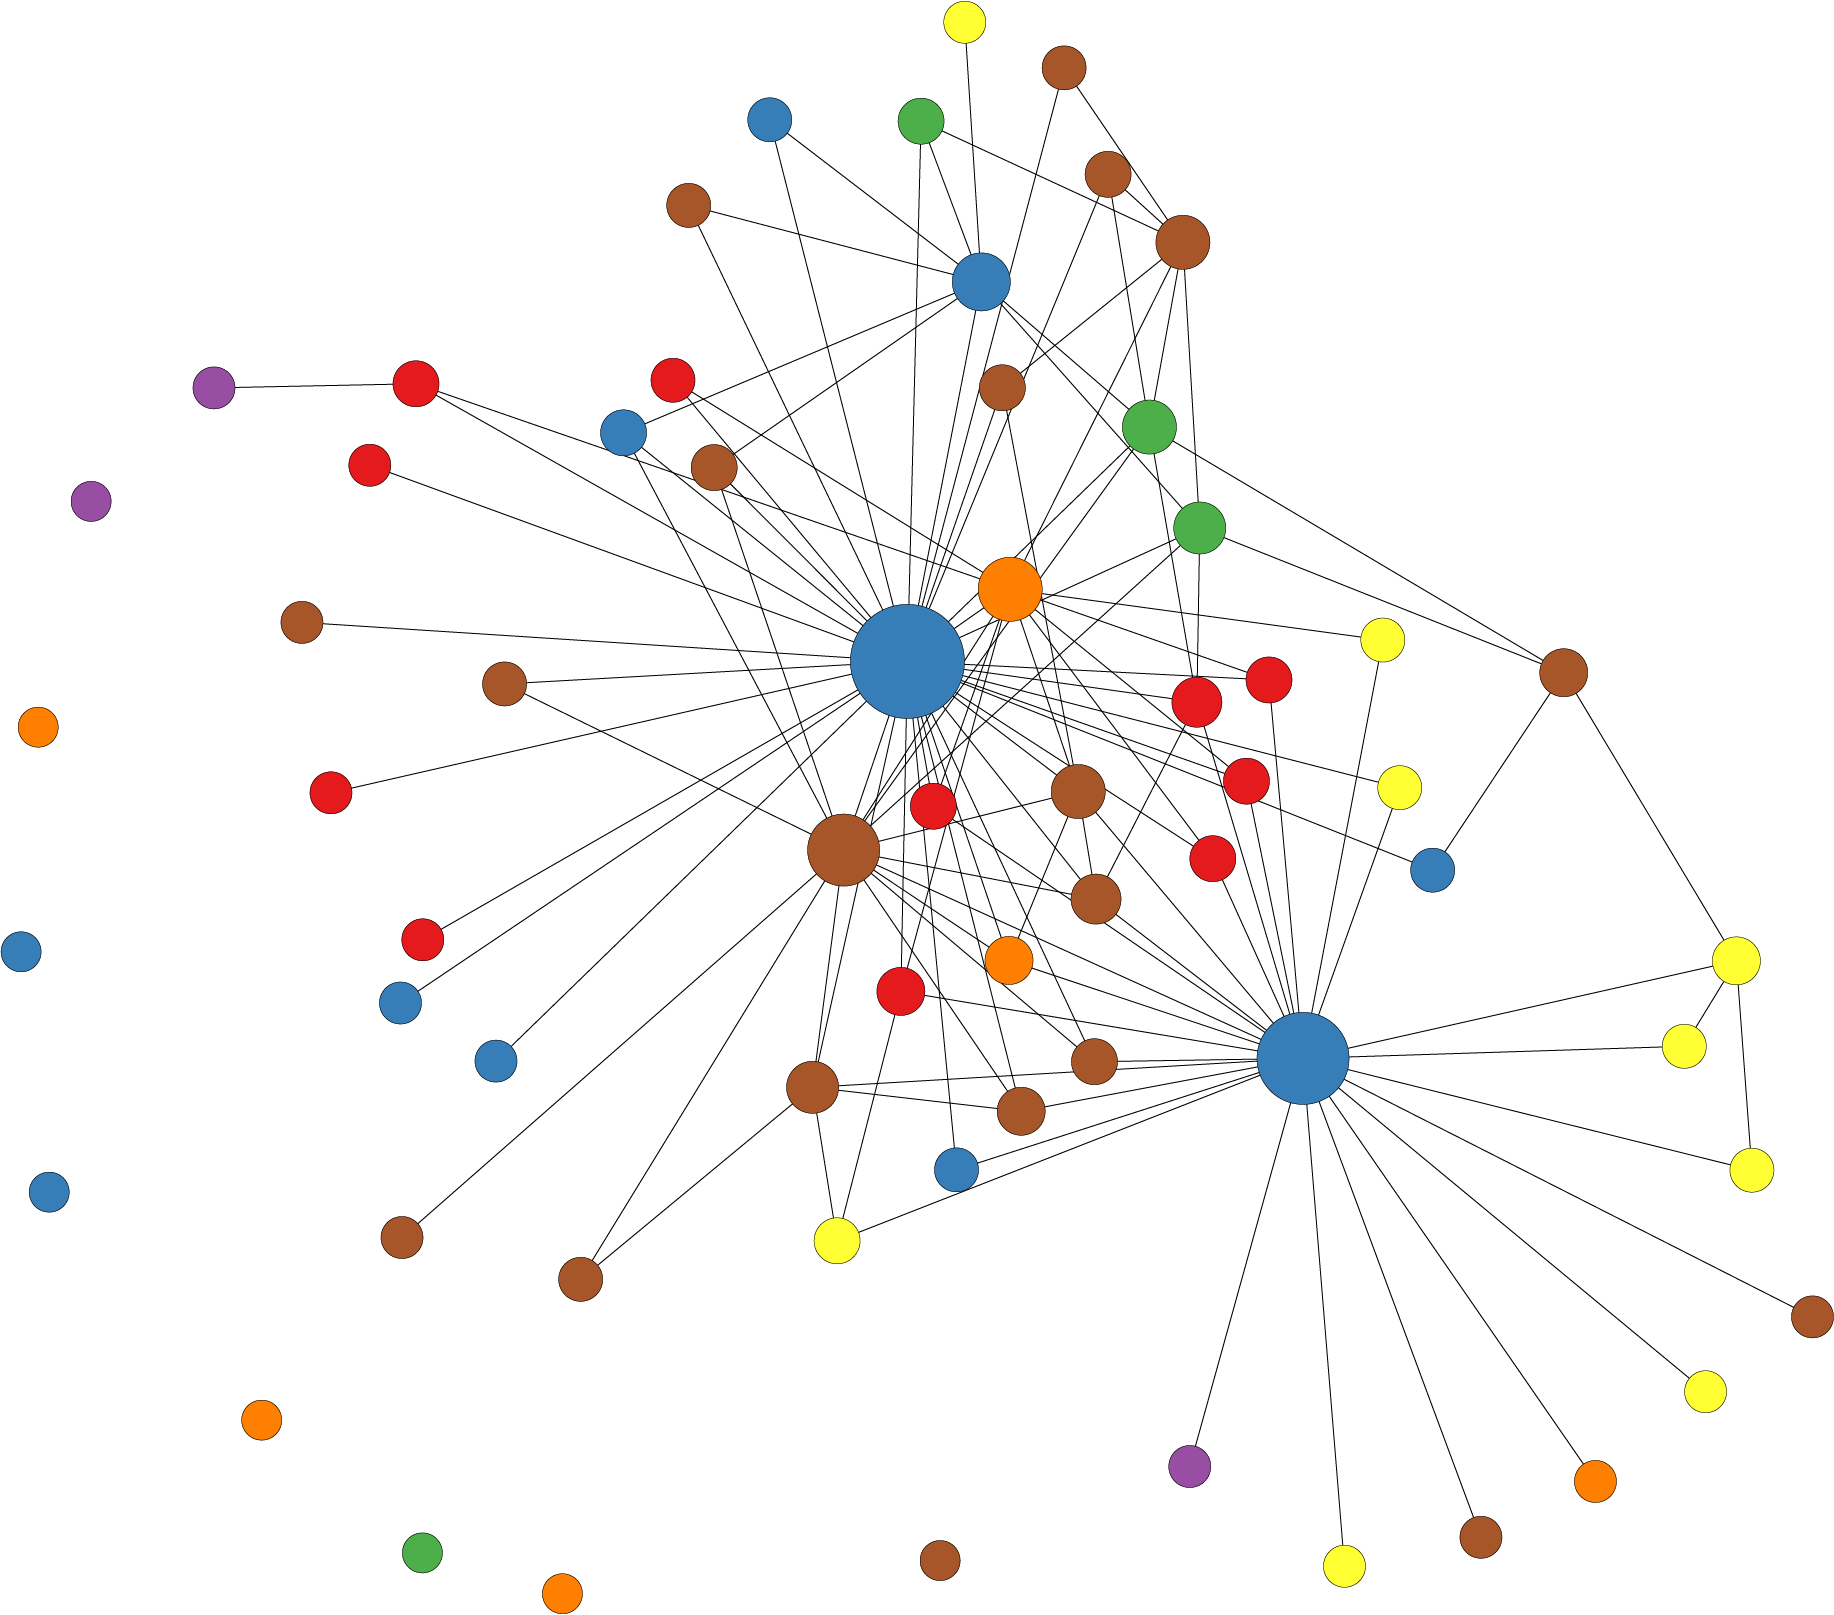
\includegraphics[width=4.0cm]{pic/logo_graph.png}
\hspace*{0.25cm}~%
% 
\includegraphics[width=1.4cm]{pic/unmsm.png}
\vspace*{0.35cm}\\

% Inteligencia Artificial PUCP (IA-PUCP)
% IA-PUCP
}

\date{\scriptsize August 28, 2025}
\usepackage{YTU}

% defs
\def\cmd#1{\texttt{\color{red}\footnotesize $\backslash$#1}}
\def\env#1{\texttt{\color{blue}\footnotesize #1}}
\definecolor{deepblue}{rgb}{0,0,0.5}
\definecolor{deepred}{rgb}{0.6,0,0}
\definecolor{deepgreen}{rgb}{0,0.5,0}
\definecolor{halfgray}{gray}{0.55}

\lstset{
    basicstyle=\ttfamily\small,
    keywordstyle=\bfseries\color{deepblue},
    emphstyle=\ttfamily\color{deepred},    % Custom highlighting style
    stringstyle=\color{deepgreen},
    numbers=left,
    numberstyle=\small\color{halfgray},
    rulesepcolor=\color{red!20!green!20!blue!20},
    frame=shadowbox,
}

\begin{document}

\begin{frame}
    \titlepage
    \begin{figure}[ht!]
        \begin{center}
            % 
\includegraphics[width=0.2\linewidth]{pic/YTU_logo.jpg}
       \end{center}
    \end{figure}
    
    \begin{note}
        {Go...}
    \end{note}
\end{frame}
    
\begin{frame}
    \tableofcontents[sectionstyle=show,subsectionstyle=show/shaded/hide,subsubsectionstyle=show/shaded/hide]
    % \tableofcontents[sectionstyle=show,subsectionstyle=hide,subsubsectionstyle=hide]
\end{frame}

\section{Introduction}
    \begin{frame}{Graph Neural Networks}
        \centering \LARGE \texttt{Graph Theory + Neural Networks}
    \end{frame}
    
    \begin{frame}{Graphs}
        Graph is a data structure and is defined as $G = (V, E)$, where $V = \{v_1, v_2, ..., v_{n}\}$ is the nodes (or \textit{vertices}, or \textit{points}) set and $E = \{e_1, e_2, ..., e_{m}\}, e_i \in V \times V$ a set of edges (or \textit{lines}, or \textit{arcs}) formed by unordered pairs of nodes. \\

        % \vspace{2mm}
        % \scriptsize Number of nodes is denoted $|V|$. \\
        % Number of edges is denoted $|E|$.
        
        \begin{figure}[ht!]
            \centering
            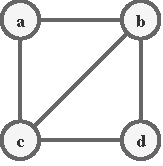
\includegraphics[width=0.25\linewidth]{pic/graph_example.pdf}
            \caption{ Graph example.}
        \end{figure}
    \end{frame}

    \begin{comment}
    \begin{frame}{Graphs}
        Furthermore, each edge $e \in E$ is said to join two vertices. If $e$ joins $u, v \in V$, then $e = (u, v)$. Vertices $u$ and $v$ are said to be adjacent. \\
        
        \begin{exampleblock}{Neighborhood}
            \begin{equation}
            N(v) = \{w \in V ∣ v \neq w, \exists \; e \in E: e = (u, v)\}
            \label{eq:neighborhood}
            \end{equation}
        \end{exampleblock}

        \begin{note}
            {Introduce your self}
        \end{note}
    \end{frame}
    \end{comment}

    \begin{frame}{Graph representations}
        \begin{figure}
            \centering
            \begin{subfigure}{0.241\textwidth}
                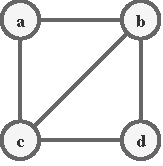
\includegraphics[width=\textwidth]{pic/graph_example.pdf}
                \caption{Input graph.}
                \label{fig:graph_example}
            \end{subfigure}
            \hfill
            \begin{subfigure}{0.241\textwidth}
                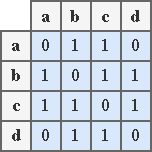
\includegraphics[width=\textwidth]{pic/graph_adjacency_matrix.pdf}
                \caption{Adjacency matrix.}
                \label{fig:second}
            \end{subfigure}
            \hfill
            \begin{subfigure}{0.241\textwidth}
                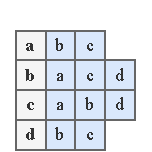
\includegraphics[width=\textwidth]{pic/graph_adjacency_list.pdf}
                \caption{Adjacency list.}
                \label{fig:graph_adjacency_list}
            \end{subfigure}
                    \hfill
            \begin{subfigure}{0.241\textwidth}
                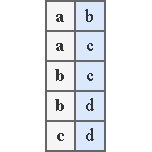
\includegraphics[width=\textwidth]{pic/graph_list_edge.pdf}
                \caption{Edge list.}
                \label{fig:graph_list_edge}
            \end{subfigure}
            \caption{Graph representations.}
            \label{fig:graph_representation}
        \end{figure}                     
    \end{frame}

    \begin{frame}{Types of graphs}
        \begin{figure}
            \centering
            \begin{subfigure}{0.241\textwidth}
                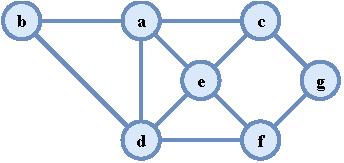
\includegraphics[width=\textwidth]{pic/homogeneous_graph.pdf}
                \caption{Homogeneous.}
                \label{fig:homogeneous_graph}
            \end{subfigure}
            \hfill
            \begin{subfigure}{0.241\textwidth}
                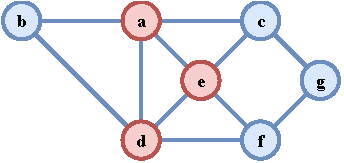
\includegraphics[width=\textwidth]{pic/heterogeneous_graph.pdf}
                \caption{Heterogeneous.}
                \label{fig:heterogeneous_graph}
            \end{subfigure}
            \hfill
            \begin{subfigure}{0.241\textwidth}
                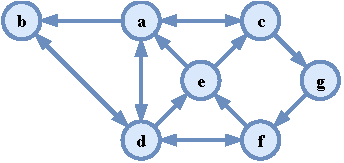
\includegraphics[width=\textwidth]{pic/directed_graph.pdf}
                \caption{Directed.}
                \label{fig:directed_graph}
            \end{subfigure}
            \hfill
            \begin{subfigure}{0.241\textwidth}
                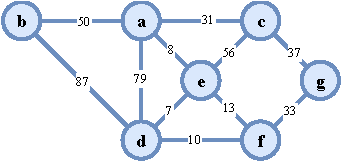
\includegraphics[width=\textwidth]{pic/weighted_undirected_graph.pdf}
                \caption{Weighted.}
                \label{fig:weighted_undirected_graph}
            \end{subfigure}
            \hfill
            \begin{subfigure}{0.16\textwidth}
                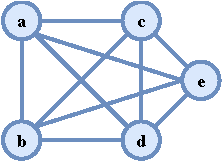
\includegraphics[width=\textwidth]{pic/complete_graph.pdf}
                \caption{Complete.}
                \label{fig:complete_graph}
            \end{subfigure}
            \hfill
            \begin{subfigure}{0.195\textwidth}
                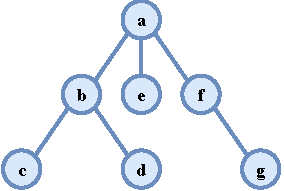
\includegraphics[width=\textwidth]{pic/tree.pdf}
                \caption{Tree.}
                \label{fig:tree}
            \end{subfigure}
            \hfill
            \begin{subfigure}{0.11\textwidth}
                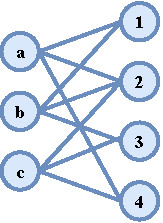
\includegraphics[width=\textwidth]{pic/2_partite_graph.pdf}
                \caption{Bipartite.}
                \label{fig:2_partite_graph}
            \end{subfigure}
            \hfill
            \begin{subfigure}{0.25\textwidth}
                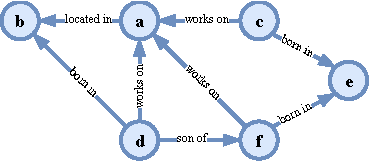
\includegraphics[width=\textwidth]{pic/knowledge_graph.pdf}
                \caption{Knowledge.}
                \label{fig:knowledge_graph}
            \end{subfigure}
            \caption{Types of graphs.}
            \label{fig:types_graphs}
        \end{figure}                     
    \end{frame}

    \begin{frame}{Graphs are everywhere!}
        \begin{figure}[ht!]
            \centering
            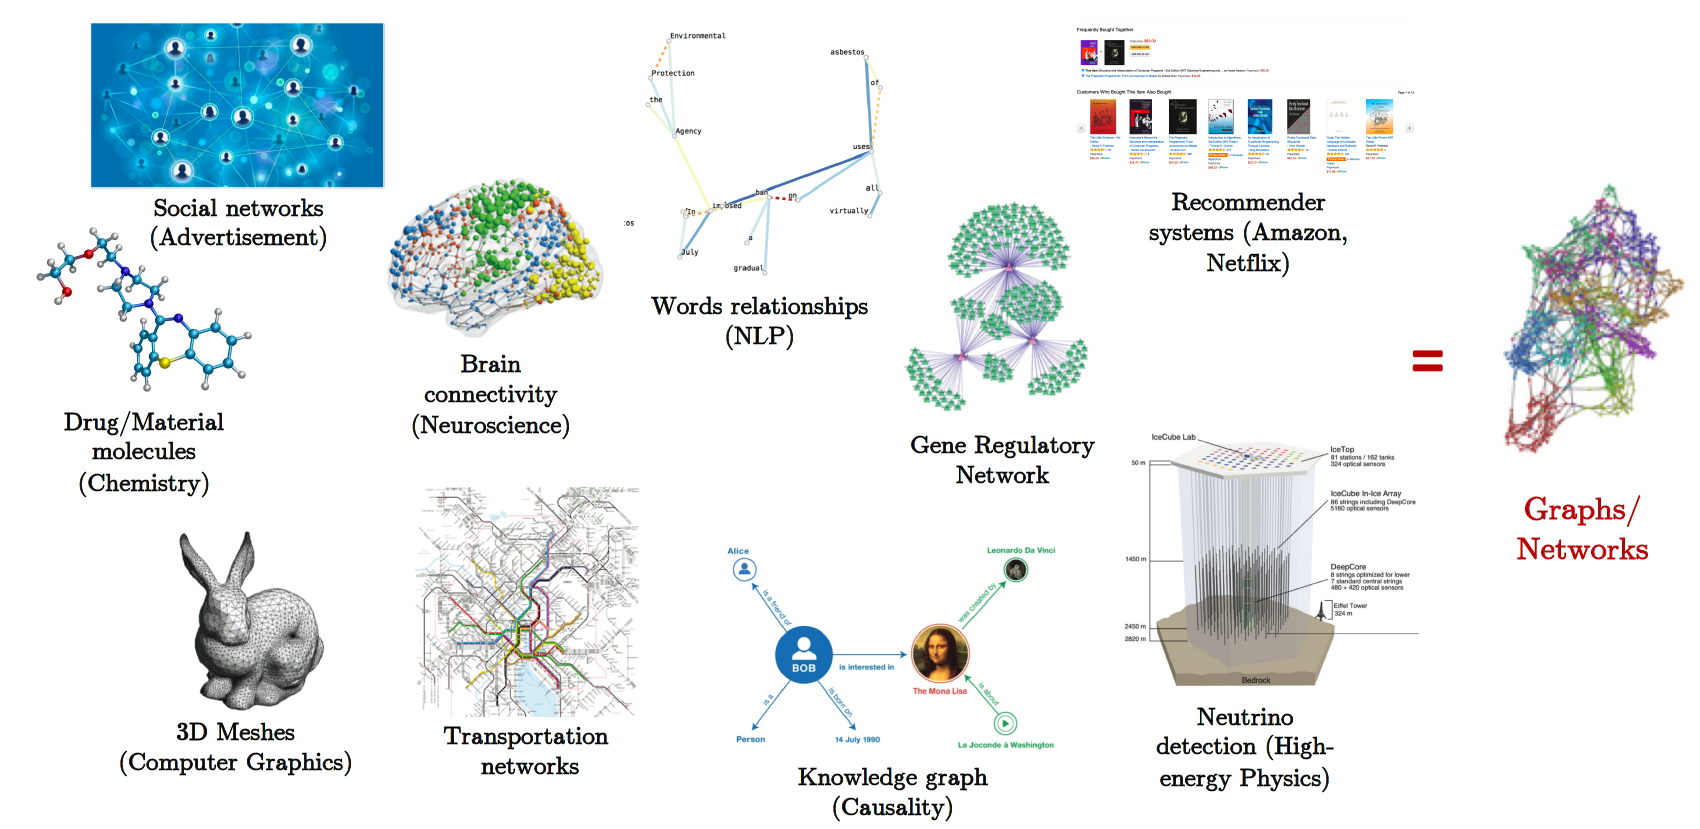
\includegraphics[width=1.0\linewidth]{pic/graph-data.png}
            \caption{\scriptsize Graphs are everywhere. From \url{https://graphdeeplearning.github.io/project/spatial-convnets/}.}
        \end{figure}               
    \end{frame}

    \begin{comment}
    \begin{frame}{Types of graphs}
        \begin{columns}[t] % The "c" centered vertical alignment, "t" top vertical alignment
            \begin{column}{0.35\textwidth}
               \begin{itemize}
                    \item \textbf{Based on nodes}
                    \begin{itemize}
                        \item Homogeneous
                        \item Heterogeneous
                    \end{itemize}
                \end{itemize}
            \end{column}
            
            \begin{column}{0.34\textwidth}
               \begin{itemize}
                    \item \textbf{Based on edges}
                    \begin{itemize}
                        \item Undirected
                        \item Directed
                        \item Unweighted
                        \item Weighted
                        \item Sparse
                        \item Dense
                    \end{itemize}
                \end{itemize}
            \end{column}

            \begin{column}{0.32\textwidth}
               \begin{itemize}
                    \item \textbf{Special types}
                    \begin{itemize}
                        \item Complete
                        \item Subgraph
                        \item Hypergraph
                        \item \textit{k}-partite
                        \item Acyclic and Cyclic
                        \item Tree
                        \item Knowledge            
                        % \item Planar
                    \end{itemize}
                \end{itemize}
            \end{column}
        \end{columns}

        \begin{note}
            {Introduce your self}
        \end{note}
    \end{frame}

    \begin{frame}{Based on nodes}         
        \begin{exampleblock}{Homogeneous graph}
            Is a graph $G = (V, E)$ in which all nodes and/or edges are of the same type, or class. %, meaning they represent entities of the same class or category, and there is no distinction.
            
            \begin{figure}[ht!]
                \centering
                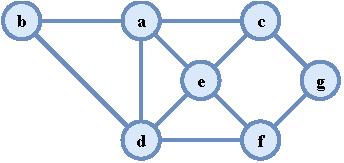
\includegraphics[width=0.4\linewidth]{pic/homogeneous_graph.pdf}
                \caption{Homogeneous graph.}
                \label{fig:homogeneous_graph}
            \end{figure}
        \end{exampleblock}
        \vspace{-2mm}

        Example: In a social network, where all vertices represent people and edges represent friendships.
        
        \begin{note}
            {Introduce your self}
        \end{note}
    \end{frame}

    \begin{frame}{Based on nodes}         
        \begin{exampleblock}{Heterogeneous graph}
            Is a graph $G = (V, E)$ in which nodes and/or edges belong to different types or classes. % In such graphs, vertices represent different kinds of entities, and edges represent different types of relationships.
            
            \begin{figure}[ht!]
                \centering
                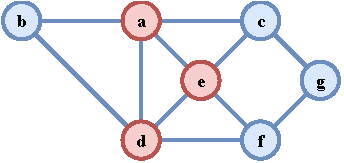
\includegraphics[width=0.4\linewidth]{pic/heterogeneous_graph.pdf}
                \caption{Heterogeneous graph.}
                \label{fig:heterogeneous_graph}
            \end{figure}
        \end{exampleblock}
        \vspace{-2mm}

        Example: In a social school network, where nodes represent teachers/students and edges represent friendships.
        
        \begin{note}
            {Introduce your self}
        \end{note}
    \end{frame}

    \begin{frame}{Based on edges}         
        \begin{exampleblock}{Directed graph (digraph)}
            Is a graph $G = (V, E)$ in which each edge has a direction. 
            An edge $(u, v)$ is not the same as $(v, u)$.
            % Formally, edges are represented as ordered pairs $(u, v)$, indicating a connection from node $u$ to node $v$. 
            % E⊆V×V is a set of ordered pairs called arcs or directed edges
            
            \begin{figure}[ht!]
                \centering
                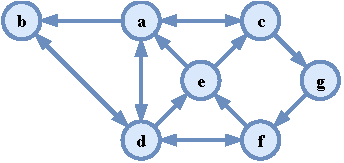
\includegraphics[width=0.4\linewidth]{pic/directed_graph.pdf}
                \caption{Directed graph.}
                \label{fig:directed_graph}
            \end{figure}
        \end{exampleblock}
        \vspace{-2mm}

        Example: commonly used to model asymmetric relationships, such as: follow relationships in social networks, task dependencies, etc.

        \begin{note}
            {Introduce your self}
        \end{note}
    \end{frame}

    \begin{frame}{Based on edges}         
        \begin{exampleblock}{Weighted graph}
            Is a graph $G = (V, E, w)$ in which each edge is assigned a numerical value, called a weight. This weight is denoted $w(u, v)$ for edge $(u, v)$.
            % $G = (V, E, w)$
            
            \begin{figure}
                \centering
                \begin{subfigure}{0.4\textwidth}
                    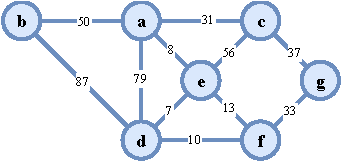
\includegraphics[width=\textwidth]{pic/weighted_undirected_graph.pdf}
                    \caption{Weighted \& undirected.}
                    \label{fig:weighted_undirected_graph}
                \end{subfigure}
                % \hfill
                \hspace{1cm}
                \begin{subfigure}{0.4\textwidth}
                    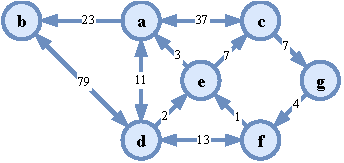
\includegraphics[width=\textwidth]{pic/weighted_directed_graph.pdf}
                    \caption{Weighted \& undirected.}
                    \label{fig:weighted_directed_graph}
                \end{subfigure}
                \caption{Weighted graph.}
                \label{fig:weighted_graph}
            \end{figure}
        \end{exampleblock}
        \vspace{-2mm}
        
        Example: commonly used in shortest path problems, network routing, road maps, cost optimization problems, etc.

        \begin{note}
            {Introduce your self}
        \end{note}
    \end{frame}

    % Complete graph
    \begin{frame}{Special types}         
        \begin{exampleblock}{Complete graph}
            % A simple graph G is complete if every pair of distinct vertices is adjacent. The complete graph on n vertices is denoted Kn.

            A complete graph $G = (V, E)$ is a simple graph in which each pair of distinct vertices is adjacent to each other. In other words, there are all possible edges between the nodes.
            
            \begin{figure}[ht!]
                \centering
                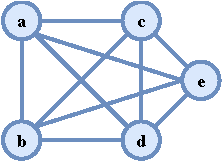
\includegraphics[width=0.27\linewidth]{pic/complete_graph.pdf}
                \caption{Complete graph.}
                \label{fig:complete_graph}
            \end{figure}
        \end{exampleblock}
        \vspace{-5mm}
        Example: In modeling networks with maximum connectivity, etc.

        \begin{note}
            {Introduce your self}
        \end{note}
    \end{frame}

    % Subgraph graph
    \begin{frame}{Special types}         
        \begin{exampleblock}{Subgraph graph}
            A subgraph of a graph $G_1 = (V_1, E_1)$ is a graph $G_2 = (V_2, E_2)$ that satisfies $V_2 \subseteq V_1$ and $E_2 \subseteq E_1$.%  \cite{saoub2021graph}.
            
            %  A subgraph H of a graph G is a graph where H contains some of the edges and vertices of G; that is, V (H) ⊆ V (G) and E(H) ⊆ E(G).

            \begin{figure}
                \centering
                \begin{subfigure}{0.41\textwidth}
                    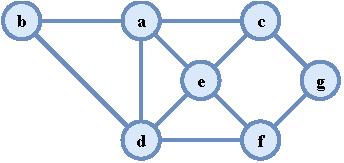
\includegraphics[width=\textwidth]{pic/homogeneous_graph}
                    \caption{Graph $G_{1}$.}
                    \label{fig:graph}
                \end{subfigure}
                % \hfill
                \hspace{1cm}
                \begin{subfigure}{0.18\textwidth}
                    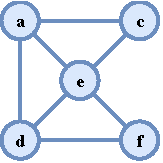
\includegraphics[width=\textwidth]{pic/subgraph.pdf}
                    \caption{Subgraph $G_{2}$.}
                    \label{fig:subgraph}
                \end{subfigure}
                \caption{Graph and subgraph.}
                \label{fig:graph_subgraph}
            \end{figure}

            % Example: In a social network, where all vertices represent people and edges represent friendships.
        \end{exampleblock}

        \begin{note}
            {Introduce your self}
        \end{note}
    \end{frame}

    % Tree
    \begin{frame}{Special types}         
        \begin{exampleblock}{Tree}
            % A simple, connected graph having no cycles is called a tree. A simple graph having only trees as its components, is called a forest.
            % For any connected (simple) graph G with n vertices and m edges, n ≤ m + 1.
            A graph $G = (V, E)$ is a tree if and only if there exists exactly one path between every two vertices $u$ and $v$.
            
            \begin{figure}[ht!]
                \centering
                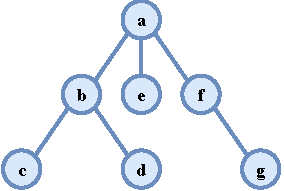
\includegraphics[width=0.37\linewidth]{pic/tree.pdf}
                \caption{Tree.}
                \label{fig:tree}
            \end{figure}
        \end{exampleblock}
        \vspace{-5mm}
        Example: In data structures, file system, machine learning, etc.

        \begin{note}
            {Introduce your self}
        \end{note}
    \end{frame}

    % Knowledge graph
    \begin{frame}{Special types}         
        \begin{exampleblock}{Knowledge graph}
            A knowledge graph (KG) is a labeled directed graph, where the nodes represent the entities and the edges represent the semantic relationships between them.
            \footnotesize KG is defined as a set of triplets: $\text{KG} = \{(s, p, o) | s \in \mathscr{E}, p \in \mathscr{R}, o \in \mathscr{E}\}$. Where, $s$ a subject (an entity), $p$ a predicate (a relation), $o$ an object (an entity), $\mathscr{E}$ set of entities (nodes), $\mathscr{R}$ set of relations (edge labels).
            
            % relationships between them.
            \begin{figure}[ht!]
                \centering
                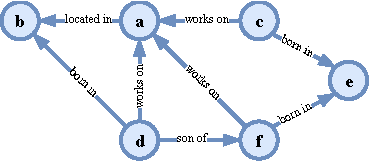
\includegraphics[width=0.45\linewidth]{pic/knowledge_graph.pdf}
                \caption{Knowledge graph.}
                \label{fig:knowledge_graph}
            \end{figure}
        \end{exampleblock}
        \vspace{-5mm}
        Example: In question-answering systems, healthcare, recommender systems, etc.
        
        \begin{note}
            {Introduce your self}
        \end{note}
    \end{frame}
    \end{comment}

    \begin{frame}{Algorithms on graphs}
        \begin{figure}
            \centering
            \begin{subfigure}{0.241\textwidth}
                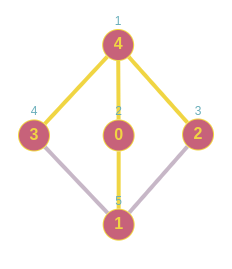
\includegraphics[width=\textwidth]{pic/bfs_v1.png}
               \caption{BFS traversal from node 4 are 4, 0, 2, 3, 1.}
                \label{fig:bfs_v1}
            \end{subfigure}
            % \hfill
            \hspace{10mm}
            \begin{subfigure}{0.241\textwidth}
                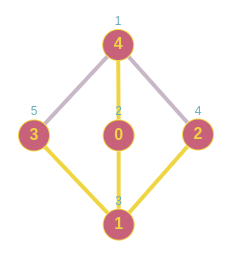
\includegraphics[width=\textwidth]{pic/dfs_v1.png}
                \caption{DFS traversal from node 4 are 4, 0, 1, 2, 3.}
                \label{fig:dfs_v1}
            \end{subfigure}
            \caption{Traversal on graphs.}
            \label{fig:alrorithm_graph}
        \end{figure}
    \end{frame}

    \begin{comment}
    \begin{frame}{Algorithms on graphs}
        \begin{columns}[t] % The "c" centered vertical alignment, "t" top vertical alignment
            \begin{column}{0.45\textwidth}
               \begin{itemize}
                    \item \textbf{Network traversal}
                    \begin{itemize}
                        \item Breadth-First Search
                        \item Depth-First Search
                    \end{itemize}
                \end{itemize}
            \end{column}
            
            \begin{column}{0.55\textwidth}
               \begin{itemize}
                    \item \textbf{Shortest path algorithms}
                    \begin{itemize}
                        \item Dijkstra
                        \item Floyd–Warshall
                        \item Bellman-Ford
                    \end{itemize}
                \end{itemize}
            \end{column}
        \end{columns}

        \begin{note}
            {Introduce your self}
        \end{note}
    \end{frame}

    \begin{frame}{Breadth-First Search (BFS) algorithm}        
        \begin{columns}[t] % The "c" option specifies centered vertical alignment while the "t" option is used for top vertical alignment
            \begin{column}{0.6\textwidth}
                \begin{enumerate}
                    \item Visit the adjacent unvisited node. Mark as visited, display, and insert (queue) in a queue.
                    \item In case no adjacent node is found, remove the first node from the queue.
                    \item Repeat steps 1, and 2 until the queue is empty.
                \end{enumerate}
            \end{column}
            
            \begin{column}{0.4\textwidth}
                \begin{figure}[ht!]
                    \centering
                    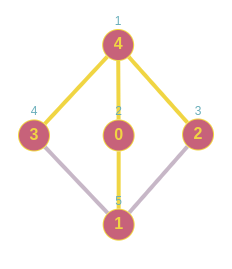
\includegraphics[width=0.8\linewidth]{pic/bfs_v1.png}
                    \caption{BFS traversal from node 4 are 4, 0, 2, 3, 1.}
                    % \caption*{Adapted from \cite{labonne2023hands}.}
                    \label{fig:bfs}
                \end{figure}
            \end{column}
        \end{columns}
        
        \begin{note}
            {Introduce your self}
        \end{note}
    \end{frame}

    \begin{frame}{Depth-First Search (DFS) algorithm}
        \begin{columns}[t] % The "c" option specifies centered vertical alignment while the "t" option is used for top vertical alignment
            \begin{column}{0.6\textwidth}
                \begin{enumerate}
                    \item Visit the adjacent unvisited node. Mark as visited, show, and push in a stack.
                    \item In case no adjacent nodes are found, all nodes in the stack that do not have adjacent nodes are popped.
                    \item Repeat steps 1, and 2 until the stack is empty.
                \end{enumerate}
            \end{column}
            
            \begin{column}{0.4\textwidth}
                \begin{figure}[ht!]
                    \centering
                    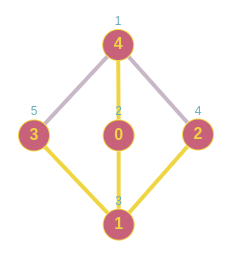
\includegraphics[width=0.7\linewidth]{pic/dfs_v1.png}
                    \caption{DFS traversal from node 4 are 4, 0, 1, 2, 3.}
                    % \caption*{Adapted from \cite{labonne2023hands}.}
                    \label{fig:dfs}
                \end{figure}
            \end{column}
        \end{columns}
        
        \begin{note}
            {Introduce your self}
        \end{note}
    \end{frame}

    \begin{frame}{Dijkstra's Algorithm}
        Dijkstra's algorithm finds the shortest path from a source node to all other nodes in a directed or undirected graph with non-negative edge weights. \newline

        \begin{exampleblock}{Idea}
            Does the shortest path from $a$ to $c$ go through $b$?
            
            \begin{figure}[ht!]
                \centering
                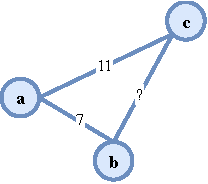
\includegraphics[width=0.25\linewidth]{pic/dijkstra_idea.pdf}
                \caption{Shortest path example.}
                \label{fig:dijkstra_idea}
            \end{figure}
        \end{exampleblock}
        
        % Description:
        % \begin{itemize}
        %    \item Uses a priority queue to select the closest unvisited node.
        %    \item Maintains the minimum known distance to each node.
        %    \item It is a weighted generalization of BFS.
        % \end{itemize}

        \begin{note}
            {Introduce your self}
        \end{note}
    \end{frame}
    \end{comment}

    \begin{comment}
    \begin{frame}{Graph measurements}
        \begin{columns}[t] % The "c" centered vertical alignment, "t" top vertical alignment
            \begin{column}{0.33\textwidth}
               \begin{itemize}
                    \item \textbf{Node-level}
                    \begin{itemize}
                        \item Degree
                        \item Degree centrality
                        \item Closeness centrality
                        \item Betweenness centrality
                        % \item Centrality
                        \item Eccentricity
                    \end{itemize}
                \end{itemize}
            \end{column}
            
            \begin{column}{0.33\textwidth}
               \begin{itemize}
                    \item \textbf{Edge-level}
                    \begin{itemize}
                        \item Shortest path
                        \item Betweenness centrality
                        \item Distance
                    \end{itemize}
                \end{itemize}
            \end{column}

            \begin{column}{0.33\textwidth}
               \begin{itemize}
                    \item \textbf{Graph-level}
                    \begin{itemize}
                        \item Order
                        \item Size
                        \item Density
                        \item Diameter
                        \item Radius
                        % \item Average path
                        \item Clustering coefficient
                        \item Modularity
                    \end{itemize}
                \end{itemize}
            \end{column}
        \end{columns}

        \begin{note}
            {Introduce your self}
        \end{note}
    \end{frame}
    \end{comment}

    \begin{frame}{Graph measurements}
        Given a graph $G = (V, E)$.

        \begin{equation}
            deg(u) = |\{v \in V : (u, v) \in E\}|
            \label{eq:degree_undirected}
        \end{equation}
        
        \begin{equation}
            deg(G) = \frac{1}{|V|}\sum_{v \in V}deg(v)
            \label{eq:degree_distribution}
        \end{equation}

        \begin{equation}
            D(G) = \frac{2|E|}{|V|(|V| - 1)}
            \label{eq:density}
        \end{equation}
        
        \begin{note}
            {Introduce your self}
        \end{note}
    \end{frame}
    
    \begin{comment}
    \begin{frame}{Node-level}
        \begin{exampleblock}{Degree}
            Given a graph $G = (V, E)$.
            
            % Number of edges incident to a node. \\

            The degree of a node $u$, denoted as $deg(u)$, is defined as the number of edges that are adjacent to this node $u$.
            
            \begin{multicols}{2} % two columns
                For undirected graphs:
                \begin{equation}
                    deg(u) = |\{v \in V : (u, v) \in E\}|
                    \label{eq:degree_undirected}
                \end{equation}
        
                For directed graphs:
                \begin{equation}
                    deg(u) = deg^{in}(u) + deg^{out}(u)
                    \label{eq:degree_directed}
                \end{equation}
            \end{multicols}
            
            Where, $deg^{in}(u)$: in-degree and $deg^{out}(u)$: out-degree. \newline

            % Degree is a measure of popularity. It determines nodes that can quickly spread information to a localized area.

        \end{exampleblock}
        \vspace{-5mm}

        Applications:
        \begin{itemize}
            \item Social networks: users with many connections.
            \item Biology networks: metabolites involved in many reactions.
            \item Web: most linked pages.
        \end{itemize}

        \begin{note}
            {Introduce your self}
        \end{note}
    \end{frame}

    \begin{frame}{Node-level}
        \begin{exampleblock}{Average degree}
            Given a graph $G = (V, E)$. \newline
            
            \begin{multicols}{2} % two columns
                The average degree of a graph $G$, denoted by $deg(G)$, is defined as the average of the degrees of all the vertices in $G$.
                \begin{equation}
                    deg(G) = \frac{1}{|V|}\sum_{v \in V}deg(v)
                    \label{eq:degree_distribution}
                \end{equation}
        
                The average degree of a graph satisfies the properties given in Equation \ref{eq:degree_distribution_property}.
                \begin{equation}
                    deg(G) = \frac{2|E|}{|V|}
                    \label{eq:degree_distribution_property}
                \end{equation}
            \end{multicols}
        \end{exampleblock}
        \vspace{-5mm}

        Applications:
        \begin{itemize}
            \item Social networks: how many friends a person has on average.
            \item Biological networks: average number of interactions per molecule.
            \item Communication networks: redundancy and connectivity estimation.
        \end{itemize}

        \begin{note}
            {Introduce your self}
        \end{note}
    \end{frame}

    \begin{frame}{Edge-level}
        \begin{exampleblock}{Shortest path}
            Given a graph $G = (V, E)$.
            
            Shortest path between two nodes in a graph is the path with the minimum total weight.
                        
        \end{exampleblock}
        \vspace{-2mm}

        Algorithms:
        \begin{itemize}
            \item Dijkstra's algorithm: for graphs with non-negative weights.
            \item Bellman-Ford: handles negative weights.
            \item Floyd-Warshall: all-pairs shortest paths.
        \end{itemize}

        Applications:
        \begin{itemize}
            \item GPS/Navigation systems: find the fastest or shortest route.
            \item Internet routing: determine optimal data transmission paths.
            \item Social networks: degrees of separation between people.
            \item Biology: identify efficient biochemical or signaling pathways.
        \end{itemize}

        % Betweenness is based on the idea that a person is more important if he/she is more intermediary in the network.

        \begin{note}
            {Introduce your self}
        \end{note}
    \end{frame}
    % add example

    \begin{frame}{Graph-level}
        \begin{exampleblock}{Order}
            Given a graph $G = (V, E)$.
            
            The order of a graph $G$, denoted by $|V|$, is defined as the number of nodes in the graph $G$.
            
        \end{exampleblock}
        % \vspace{-5mm}

        \begin{note}
            {Introduce your self}
        \end{note}
    \end{frame}

    \begin{frame}{Graph-level}
        \begin{exampleblock}{Size}
            Given a graph $G = (V, E)$.
            
            The size of a graph $G$, denoted by $|E|$, is defined as the number of edges in the graph $G$.
            
        \end{exampleblock}
        % \vspace{-5mm}

        \begin{note}
            {Introduce your self}
        \end{note}
    \end{frame}
    
    \begin{frame}{Graph-level}
        \begin{exampleblock}{Density}
            Given a graph $G = (V, E)$
            
            Density is defined as the number of network edges divided by the maximum possible number of edges between nodes in that network. All density values are between $0$ and $1$.

            \begin{equation}
                D(G) = \frac{2|E|}{|V|(|V| - 1)}
                \label{eq:density}
            \end{equation}
            
        \end{exampleblock}
        % \vspace{-5mm}

        Applications:
        \begin{itemize}
            \item Comparing different networks.
            \item Analyzing how sparse or dense a system is.
        \end{itemize}
        
        \begin{note}
            {Introduce your self}
        \end{note}
    \end{frame}
    \end{comment}
    
% \end{comment}  
% \begin{comment}
    \begin{frame}{Basics of Neural networks (NN)}
        \begin{figure}
            \centering
            % \includegraphics{}
            \animategraphics[width=0.9\textwidth, loop, autoplay]
            {10} % frame rate
            {pic/NNs/8152e79cc88f4258ad55f36b09702b35uXiAdsEiqJ6Ws9wJ-} % path to figures
            {0} % start index
            {374} % end index
            \caption{Basic NNs.}% From \url{https://www.3blue1brown.com/lessons/neural-networks}.}
            \label{fig:basic_nns}
        \end{figure}
    \end{frame}

    \begin{comment}
    \begin{frame}{Basics of Neural networks (NN)}
        \begin{figure}[ht!]
            \centering
            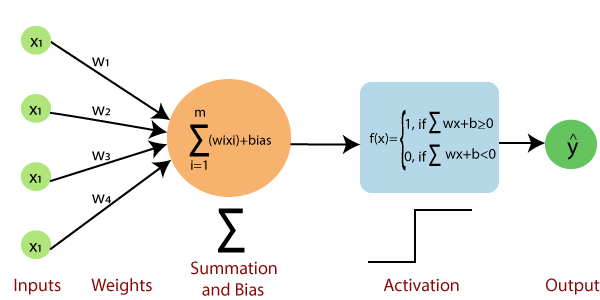
\includegraphics[width=0.86\linewidth]{pic/single-layer-perceptron-in-tensorflow2.png}
            \caption{\scriptsize Basic NN. \\
            From \url{https://www.javatpoint.com/single-layer-perceptron-in-tensorflow}.}
        \end{figure}   
    \end{frame}
    \end{comment}

    \begin{frame}{Neural networks (NN)}
        \begin{figure}[ht!]
            \centering
            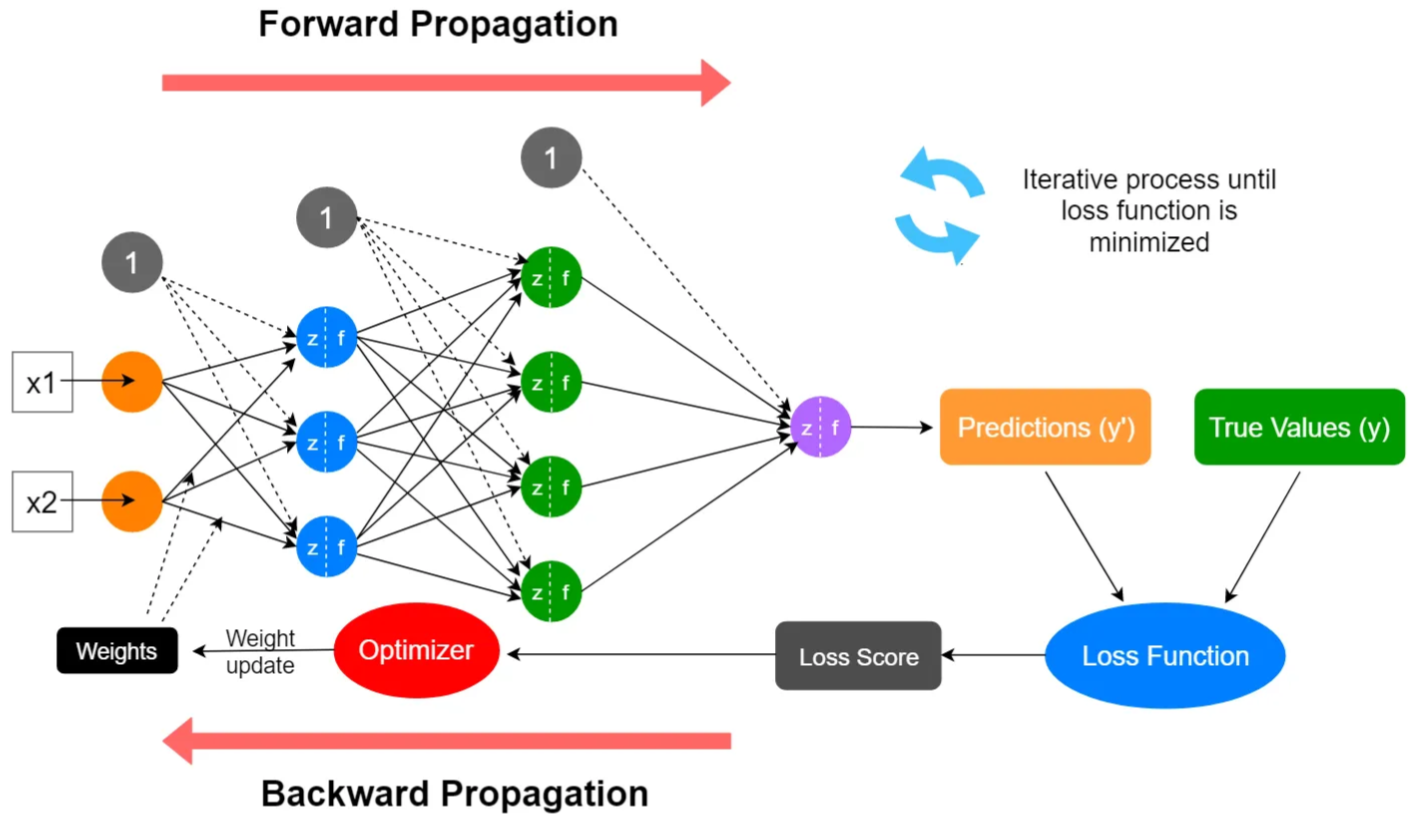
\includegraphics[width=1.0\linewidth]{pic/neural_networks.png}
            \caption{Neural networks learning. From \url{https://medium.com/data-science-365/overview-of-a-neural-networks-learning-process-61}.}
        \end{figure}   
    \end{frame}

    \begin{frame}{Example of NN}
        \begin{figure}
            \centering
            % \includegraphics{}
            \animategraphics[width=1.0\textwidth, loop, autoplay]
            {5} % frame rate
            {pic/network-propagation/network-propagation_} % path to figures
            {0} % start index
            {71} % end index
            \caption{Image classification. From \url{https://www.3blue1brown.com/lessons/neural-networks}.}
            \label{fig:example_nn}
        \end{figure}
    \end{frame}

\section{Graph Neural Networks}
    \begin{frame}{Graph embedding}
        It is a function $f: A \rightarrow Z$ that maps each node of the graph $G = (V, E)$ into a $d$-dimensional vector. Where, $Z = \{z_1, z_2, ..., z_{|V|}\}$, $z_i \in \mathbb{R}^{d}$ with $d \ll |V|$. % Usually, $z_i$ and $Z$ are called node embedding and embedding matrix, respectively.

        \begin{figure}[ht!]
            \centering
            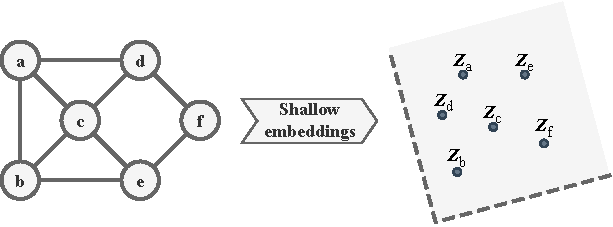
\includegraphics[width=0.7\linewidth]{pic/shallow_embeddings.pdf}
            \caption{\scriptsize Shallow embeddings scheme.}
        \end{figure}               
    \end{frame}

    \begin{frame}{Graph Neural Networks (GNN)}
        It is a function $f: (A, X) \rightarrow Z$ that maps each node of the graph $G = (V, E)$ into a $F$-dimensional vector. Where, $Z = \{z_1, z_2, ..., z_{|V|}\}$, $z_i \in \mathbb{R}^{d}$ with $d \ll |V|$.
        % \newline
        % Here, $A \in \mathbb{R}^{N \times N}$,  $X \in \mathbb{R}^{N \times C}$, $H^{l} \in \mathbb{R}^{N \times F}$ with $F \ll N$, $l \in \{1, 2, ..., L\}$.
        
        % Usually, $z_i$ and $Z$ are called node embedding and embedding matrix, respectively.
        % \centering
        % $H = \text{GNN}(A, X)$
        
        \begin{figure}[ht!]
            \centering
            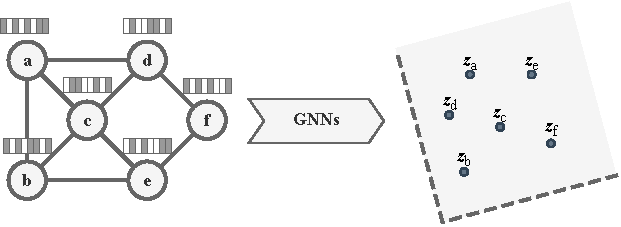
\includegraphics[width=0.7\linewidth]{pic/graph_neural_networks.pdf}
            \caption{\scriptsize GNNs scheme.}
        \end{figure}               
    \end{frame}

    \begin{frame}{How GNNs works?}
        \begin{figure}[ht!]
            \centering
            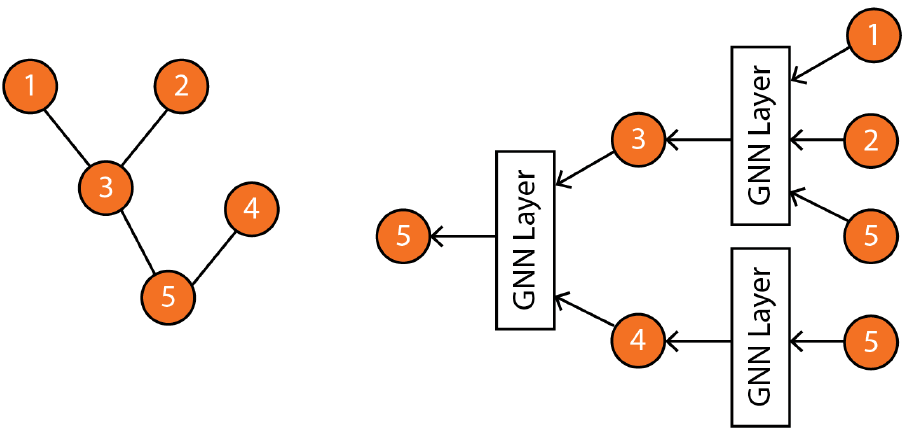
\includegraphics[width=0.7\linewidth]{pic/gnn_works.png}
            \caption{\scriptsize Computation graph representation. Adapted from \cite{labonne2023hands}.}
        \end{figure}               
    \end{frame}

    \begin{frame}{More about embeddings}
        \begin{figure}[ht!]
            \centering
            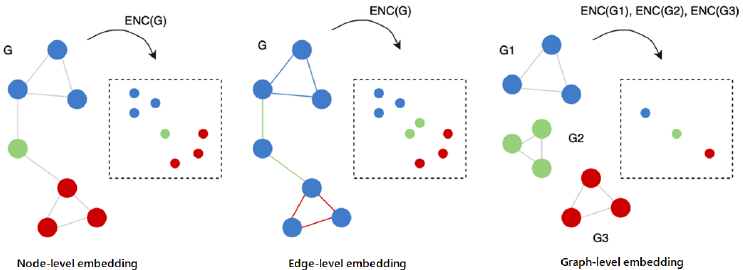
\includegraphics[width=1.0\linewidth]{pic/more_embeddings.png}
            \caption{\scriptsize Visual representation of the three different levels of granularity in graphs. Adapted from \cite{stamile2021graph}.}
        \end{figure}
                      
    \end{frame}

    \begin{frame}{Tasks}
        \begin{figure}[ht!]
            \centering
            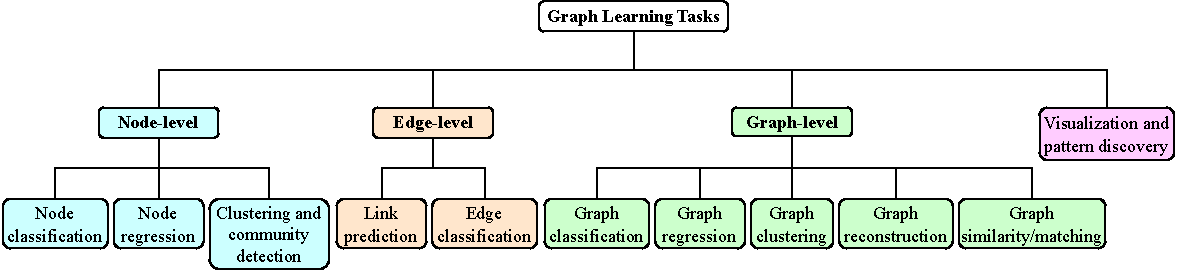
\includegraphics[width=1.0\linewidth]{pic/graph_learning_tasks.pdf}
            \caption{\scriptsize Overview of graph learning tasks.}
        \end{figure}               
    \end{frame}

    \begin{frame}{Tasks}
        \begin{figure}[ht!]
            \centering
            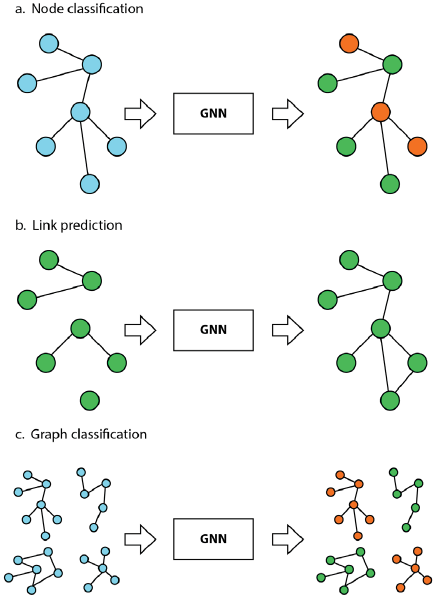
\includegraphics[width=0.43\linewidth]{pic/graph_learning_tasks_example.png}
            \caption{\scriptsize Examples of graph learning tasks. Adapted from \cite{labonne2023hands}.}
        \end{figure}               
    \end{frame}

    \begin{frame}{Node classification tasks}
        \begin{figure}
            \centering
            \begin{subfigure}{0.241\textwidth}
                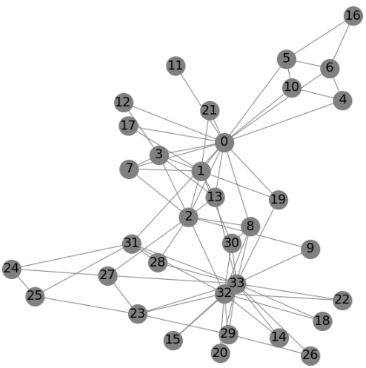
\includegraphics[width=1.0\textwidth]{pic/input_graph.png}
                \caption{\scriptsize Input graph.}
                \label{fig:input_graph_}
            \end{subfigure}
            \hfill
            \begin{subfigure}{0.241\textwidth}
                \centering
            % \includegraphics{}
            \animategraphics[width=1.3\textwidth, loop, autoplay]
            {5} % frame rate
            {pic/train_gcn/download_} % path to figures
            {0} % start index
            {149} % end index
            \caption{Train GCN.}
            \label{fig:my_label}
            \end{subfigure}
            \hfill
            \begin{subfigure}{0.241\textwidth}
                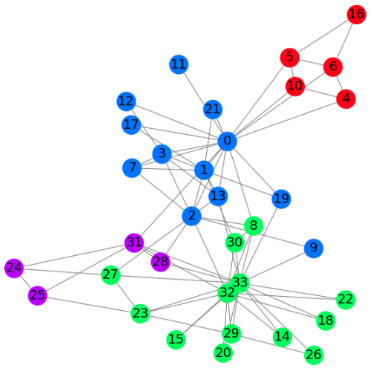
\includegraphics[width=\textwidth]{pic/output_graph.png}
                \caption{\scriptsize Output graph.}
                \label{fig:output_graph}
            \end{subfigure}
            \caption{\scriptsize GNN to node classification.}
            \label{fig:node_classification}
        \end{figure}                     
    \end{frame}

    \begin{frame}{Taxonomy of graph machine learning methods.}
        \begin{figure}[ht!]
            \centering
            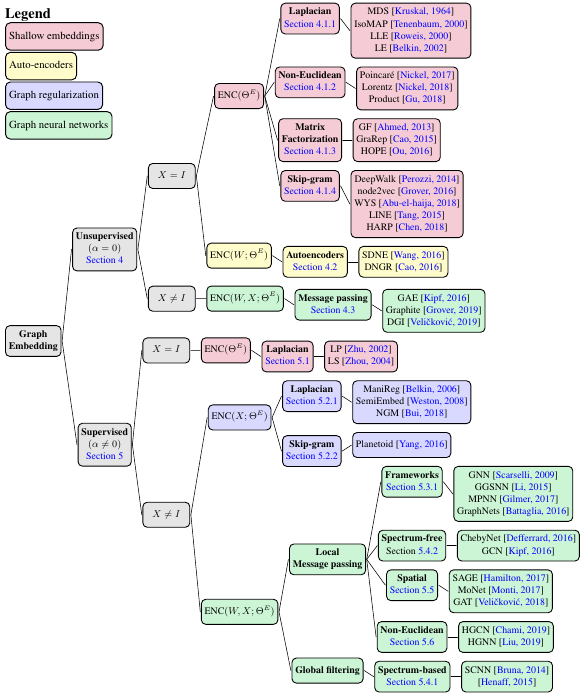
\includegraphics[width=0.512\linewidth]{pic/taxonomy_graph_machine_learning.png}
            \caption{\scriptsize Taxonomy of graph machine learning. Adapted from \cite{chami2022machine}.}
        \end{figure}               
    \end{frame}

    \begin{frame}{Variants of GNNs}
        \begin{itemize}
            \item Graph Convolutional Networks (\texttt{GCN}) \cite{kipf2016semi}
            % \item Graph Recurrent Networks (GRN)
            \item Graph Attention Networks (\texttt{GAT}) \cite{velickovic2017graph}
            \item Graph Isomorphism Networks (\texttt{GIN}) \cite{xu2018powerful}
            
            \item Variational Graph Auto-Eencoders (\texttt{VGAE}) \cite{kipf2016variational}
            \item Deep Graph Infomax (\texttt{DGI}) \cite{velivckovic2018deep}
            \item Adversarially Regularized Variational Graph Autoencoder (\texttt{ARVGA}) \cite{pan2018adversarially}
            \item Linear Graph Variational Autoencoder (\texttt{LGVAE}) \cite{salha2021simple}
            \item ...
        \end{itemize}
    \end{frame}
    
\section{Applications}
    \begin{frame}{Applications}
        \begin{multicols}{2}
            \begin{itemize}
                \item Computer vision
                \item Natural language processing
                \item Recommender systems
                \item Program analysis
                \item Knowledge graphs
                \item Bioinformatics
                \item Chemistry
                \item Biology
                \item Physic
                \item Anomaly detection
                \item Urban intelligence
                \item Financial transaction
                \item ...
            \end{itemize}
        \end{multicols}          
    \end{frame}

    \begin{comment}
    \begin{frame}{Word2vec \cite{mikolov2013efficient}}
        \begin{figure}
            \centering
            \begin{subfigure}{0.4\textwidth}
                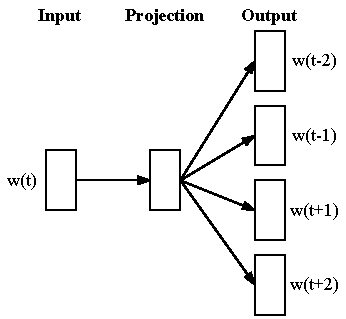
\includegraphics[width=\textwidth]{pic/skip_gram.pdf}
                \caption{\tiny Skip-gram.}
                \label{fig:first}
            \end{subfigure}
            \hfill
            \begin{subfigure}{0.4\textwidth}
                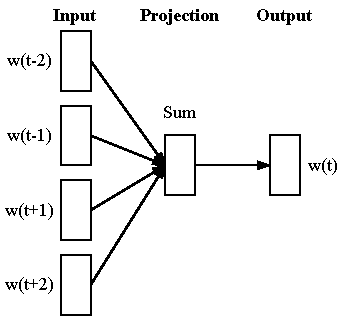
\includegraphics[width=\textwidth]{pic/cbow.pdf}
                \caption{\tiny CBOW.}
                \label{fig:third}
            \end{subfigure}
            \caption{\scriptsize Word embedding architectures. Adapted from \cite{mikolov2013efficient}.}
            \label{fig:word2vec_arquitecture}
        \end{figure} 
    \end{frame}
    \end{comment}

    \begin{comment}
    \begin{frame}{Word2vec \cite{mikolov2013efficient}}
        \begin{figure}[ht!]
            \centering
            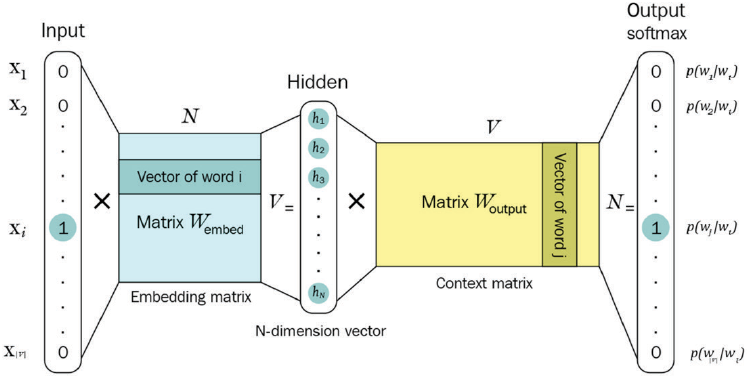
\includegraphics[width=0.9\linewidth]{pic/word2vec.png}
            \caption{\scriptsize Word2vec architecture. Adapted from \cite{labonne2023hands}.}
        \end{figure}   
    \end{frame}

    \begin{frame}{Word2vec in action}   
        \begin{figure}[ht!]
            \centering
            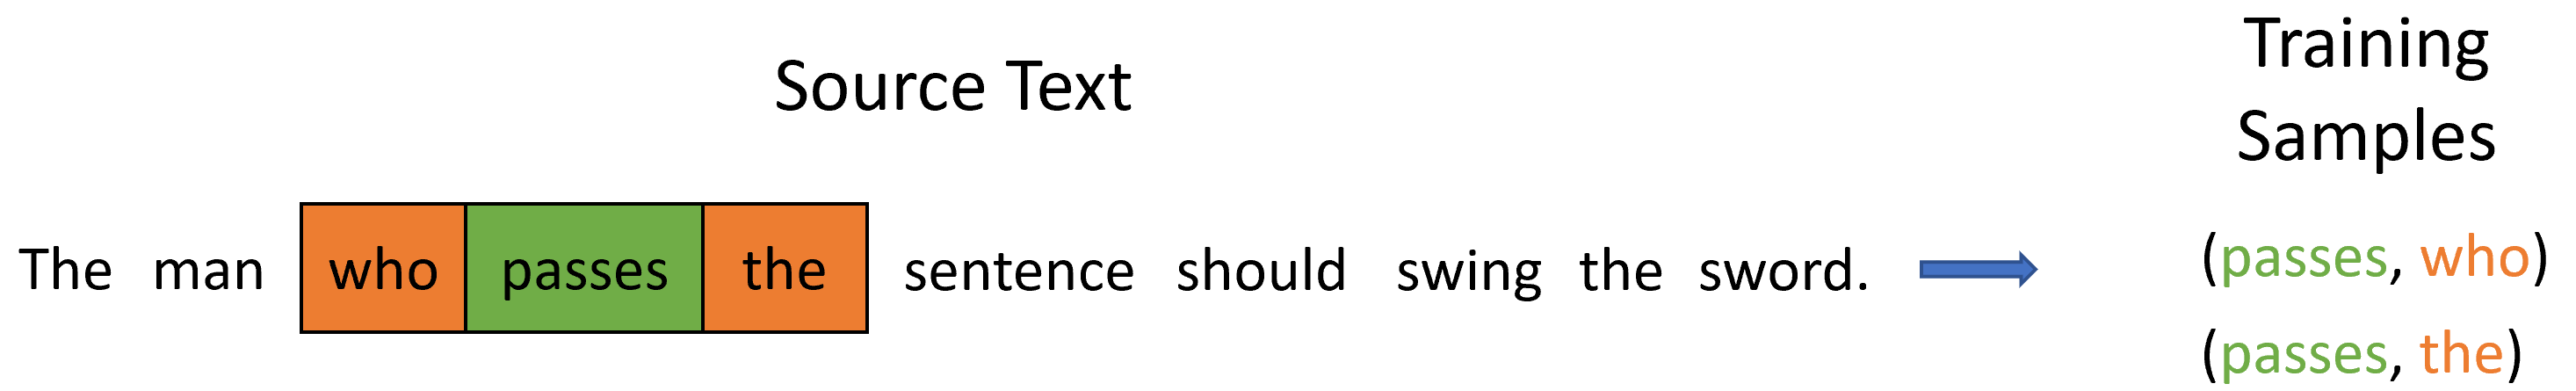
\includegraphics[width=0.65\linewidth]{pic/quote_ned_stark.png}
            \caption{\scriptsize Train window.}
        \end{figure}

        \begin{figure}[ht!]
            \centering
            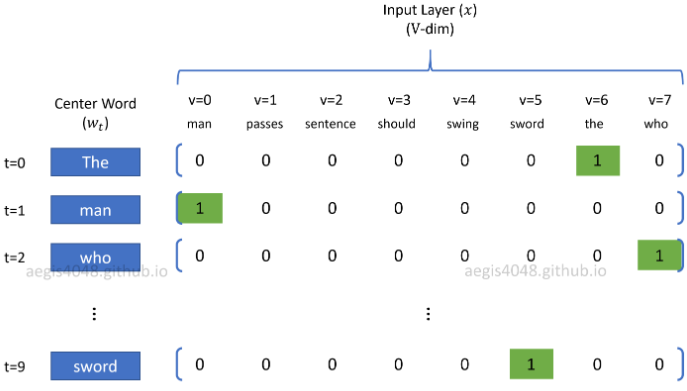
\includegraphics[width=0.7\linewidth]{pic/input_onehot.png}
            \caption{\scriptsize One-hot encoded input vector.}
        \end{figure} 
    \end{frame}

    \begin{frame}{Word2vec in action}   
        \begin{figure}[ht!]
            \centering
            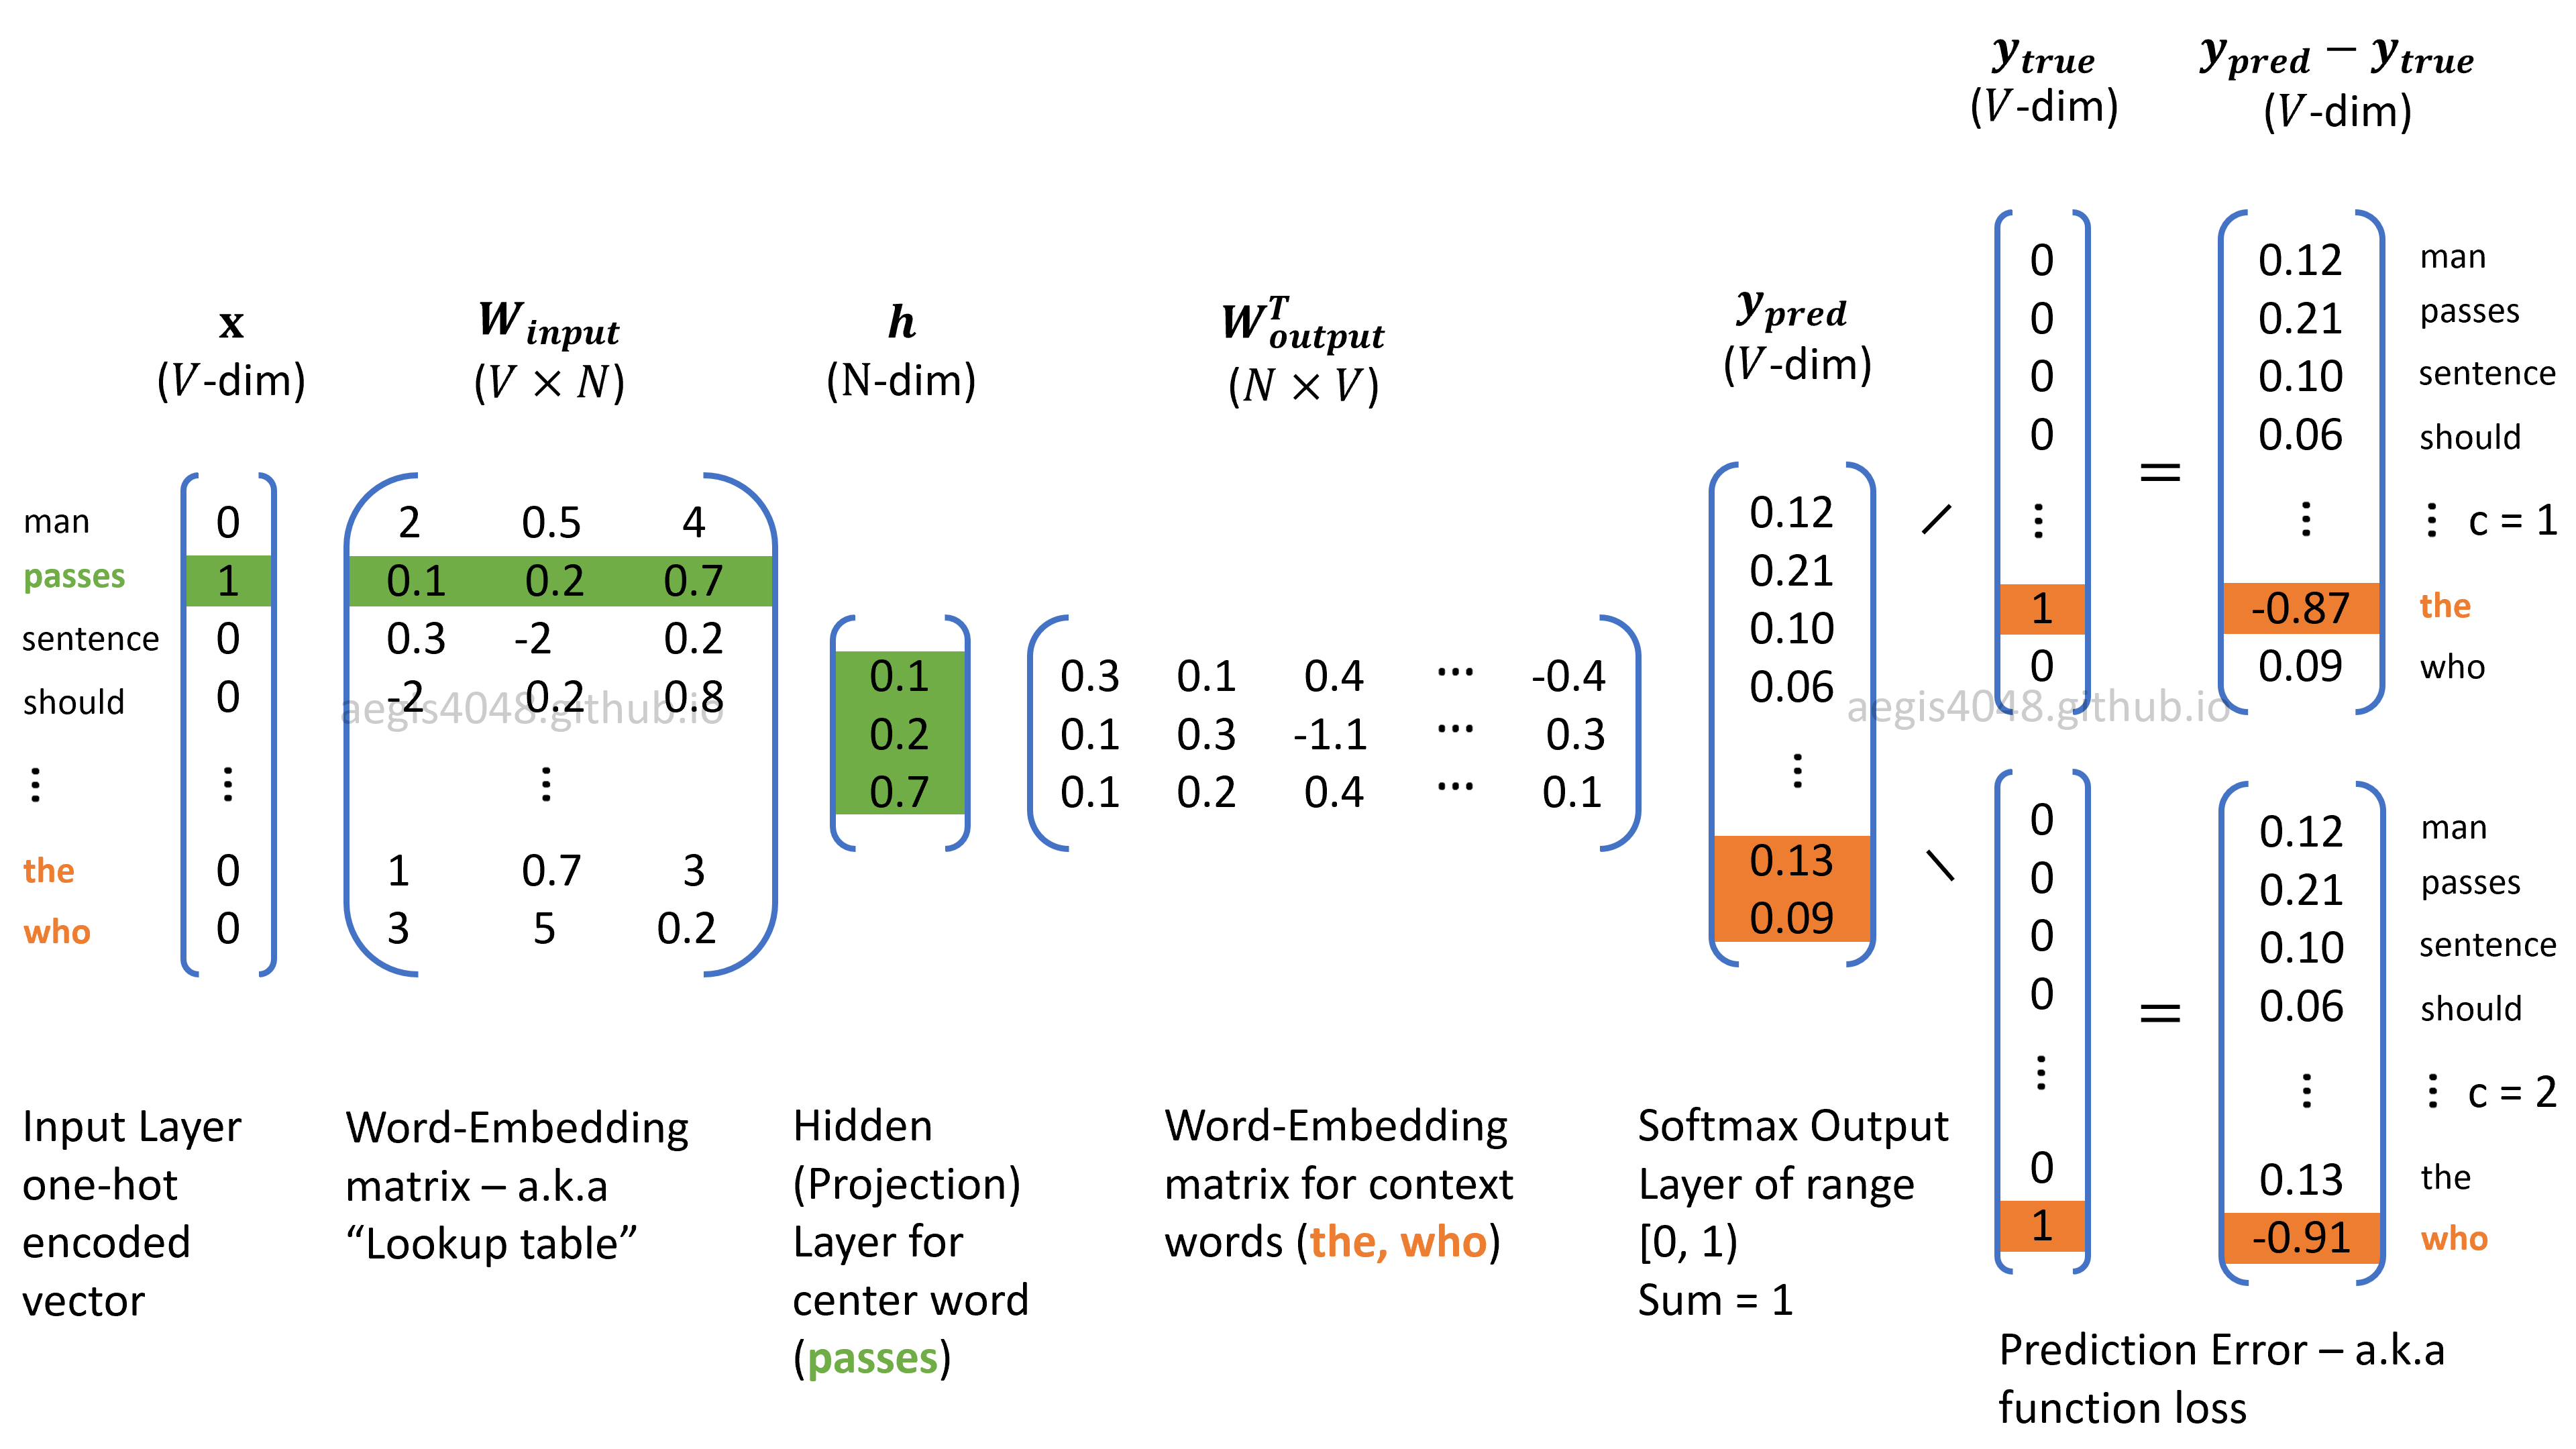
\includegraphics[width=1.0\linewidth]{pic/word2vec_skip-gram.png}
            \caption{\scriptsize Skip-Gram model structure. Current center word is ``passes''. From \url{https://aegis4048.github.io/demystifying_neural_network_in_skip_gram_language_modeling}.}
        \end{figure}   
    \end{frame}

    \begin{frame}{Word2vec in action}   
        \begin{figure}[ht!]
            \centering
            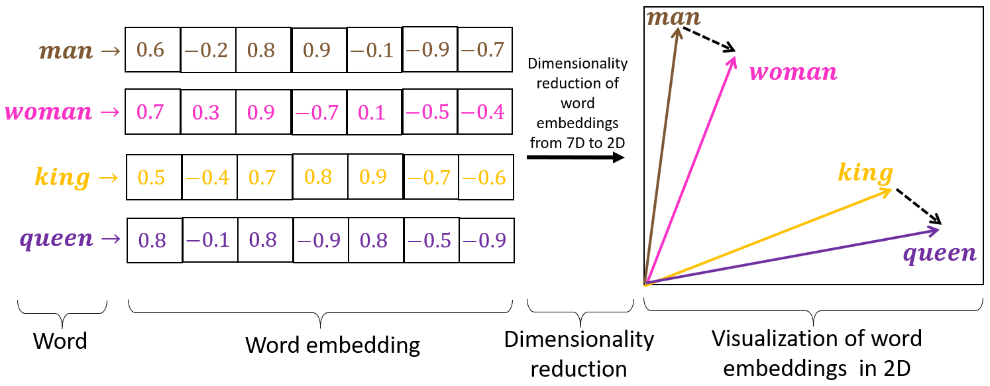
\includegraphics[width=0.85\linewidth]{pic/skip-gram_result.png}
            \caption{\scriptsize Word embeddings. \\
            From \url{https://doi.org/10.1371/journal.pone.0231189.g008}.}
        \end{figure}

        \centering
        Cosine similarity
        \begin{equation}
            cos(\theta) = \text{sim}(z_i, z_j) = \frac{z_i.z_j}{\|z_i\|\|z_j\|}
            \label{eq:cosine_similarity}
        \end{equation}
    \end{frame}

    \begin{frame}{DeepWalk \cite{mikolov2013distributed}}
        \begin{figure}[ht!]
            \centering
            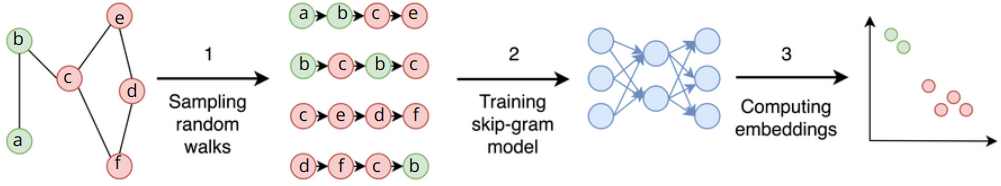
\includegraphics[width=1.0\linewidth]{pic/deepwalk.png}
            \caption{\scriptsize DeepWalk workflow.}
        \end{figure}

        Parameters:
        \begin{itemize}
            \item length = 4
            \item n = 1
        \end{itemize}
    \end{frame}

    \begin{frame}{Node2vec \cite{grover2016node2vec}} 
        \begin{figure}[ht!]
            \centering
            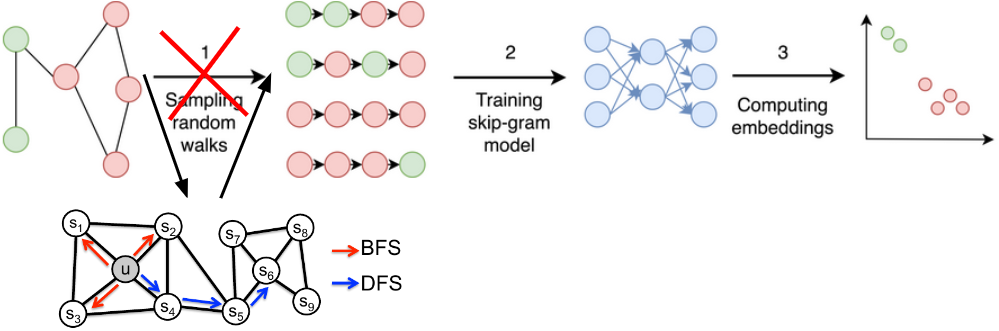
\includegraphics[width=1.0\linewidth]{pic/node2vec.png}
            \caption{\scriptsize Node2vec workflow.}
        \end{figure}

        Parameters:
        \begin{itemize}
            \item length = 4
            \item n = 1
            \item p = 1, q = 2 (BFS: micro-view) or
            \item p = 1, q = 0.5 (DFS: macro-view)
        \end{itemize}
    \end{frame}

    \end{comment}

    \begin{comment}
    \begin{frame}{Application on biomedical data} 
        \begin{figure}[ht!]
            \centering
            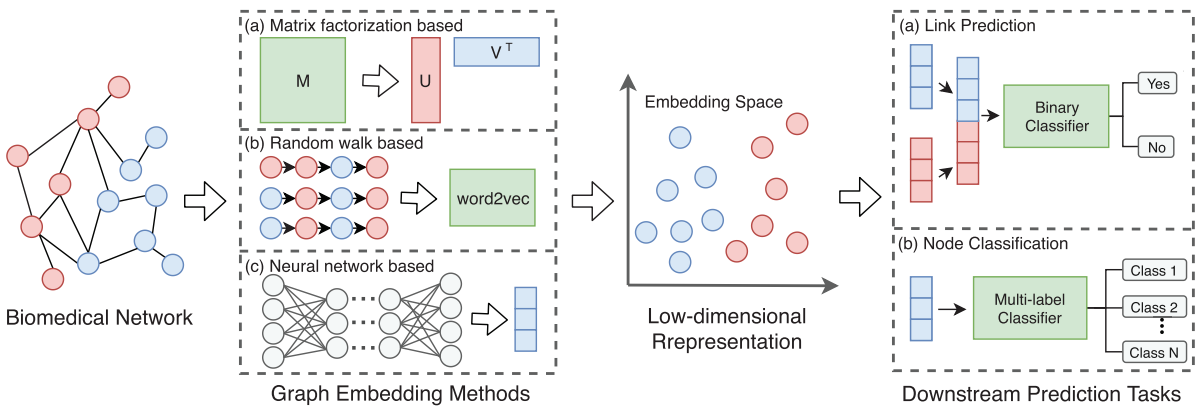
\includegraphics[width=1.0\linewidth]{pic/apply_graph_embedding.png}
            \caption{\scriptsize Applying graph embedding methods to biomedical tasks. Adapted from \cite{yue2020graph}.}
        \end{figure}
    \end{frame}    

    \begin{frame}{Graph Neural Networks (GNN)}
        It is a function $f: (A, X) \rightarrow H$ that maps each node of the graph $G = (V, E)$ into a $F$-dimensional vector. 
        \newline
        Here, $A \in \mathbb{R}^{N \times N}$,  $X \in \mathbb{R}^{N \times C}$, $H^{l} \in \mathbb{R}^{N \times F}$ with $F \ll N$, $l \in \{1, 2, ..., L\}$.
        
        % Usually, $z_i$ and $Z$ are called node embedding and embedding matrix, respectively.
        \centering
        $H = \text{GNN}(A, X)$
        \begin{figure}[ht!]
            \centering
            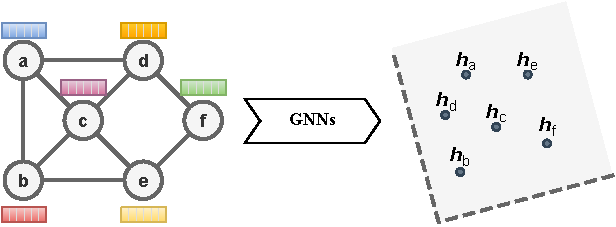
\includegraphics[width=0.7\linewidth]{pic/gnns.pdf}
            \caption{\scriptsize GNNs scheme.}
        \end{figure}               
    \end{frame}

    \begin{frame}{How GNNs works?}
        \begin{figure}[ht!]
            \centering
            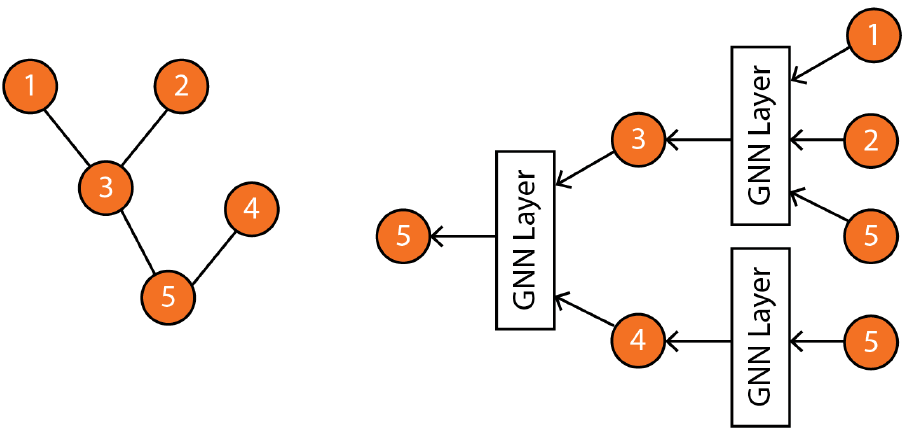
\includegraphics[width=0.7\linewidth]{pic/gnn_works.png}
            \caption{\scriptsize Computation graph representation. Adapted from \cite{labonne2023hands}.}
        \end{figure}               
    \end{frame}

    \begin{frame}{Tasks}
        \begin{figure}[ht!]
            \centering
            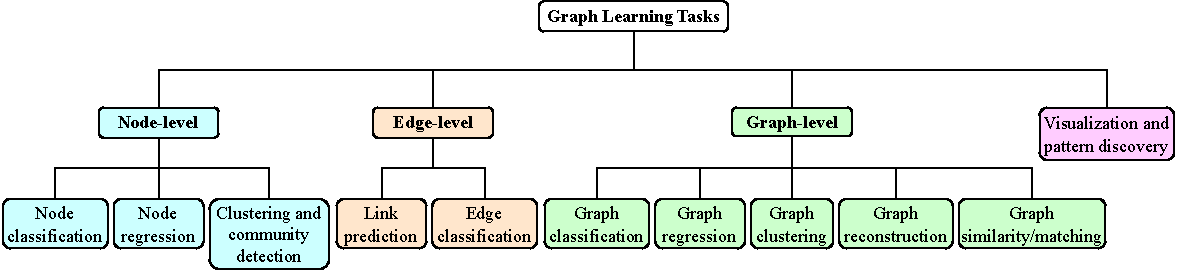
\includegraphics[width=1.0\linewidth]{pic/graph_learning_tasks.pdf}
            \caption{\scriptsize Overview of graph learning tasks.}
        \end{figure}               
    \end{frame}

    \begin{frame}{Taxonomy of graph machine learning methods.}
        \begin{figure}[ht!]
            \centering
            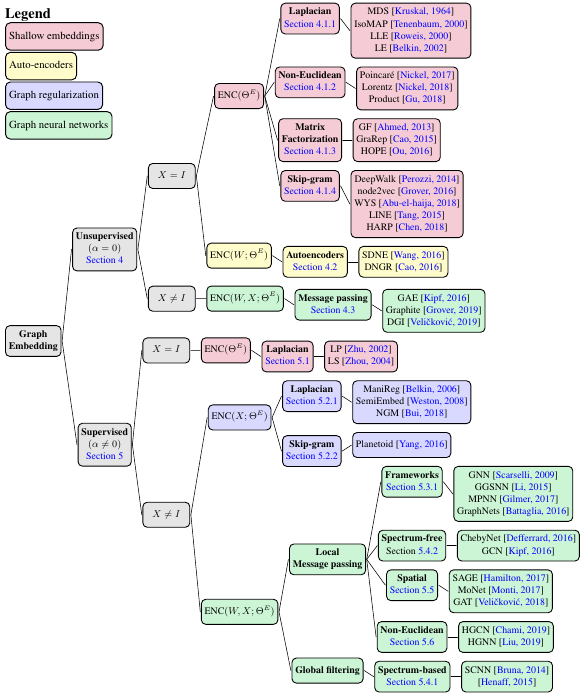
\includegraphics[width=0.512\linewidth]{pic/taxonomy_graph_machine_learning.png}
            \caption{\scriptsize Taxonomy of graph machine learning. Adapted from \cite{chami2022machine}.}
        \end{figure}               
    \end{frame}

    \end{comment}

    \begin{comment}
    \begin{frame}{Graph Convolutional Network (GCN)}
        \begin{figure}[ht!]
            \centering
            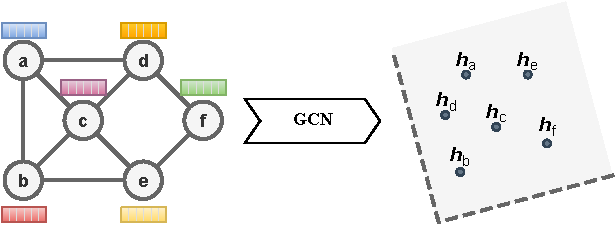
\includegraphics[width=0.7\linewidth]{pic/gcn.pdf}
            \caption{\scriptsize GCN scheme.}
        \end{figure}

        \begin{equation}
            H^{(l + 1)} = \sigma (\Tilde{D}^{-\frac{1}{2}} \Tilde{A} \Tilde{D}^{-\frac{1}{2}} H^{(l)} W^{(l)}) 
            \label{eq:propagation_gcn}
        \end{equation}

        Here, $\Tilde{A} = A + I_N$, $\Tilde{D}_{ii} = \sum_{j} \Tilde{A}_{ij}$, $W^{(l)}$ is trainable weight matrix, $\sigma(.)$ is an activation function.
    \end{frame}
    \end{comment}
    
    \begin{frame}{Application in computer vision}
        SuperGlue: Learning Feature Matching with Graph Neural Networks \cite{sarlin2020superglue}.
        
        \begin{figure}[ht!]
            \centering
            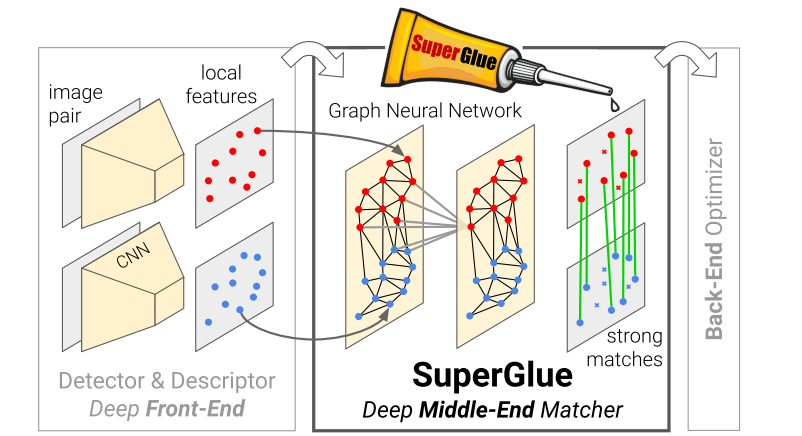
\includegraphics[width=0.7\linewidth]{pic/super_glue.png}
            \caption{SuperGlue scheme.}
        \end{figure}
    \end{frame}
    
    \begin{frame}{SuperGlue}
        \begin{figure}
            \centering
            % \includegraphics{}
            \animategraphics[width=\textwidth, loop, autoplay]
            {5} % frame rate
            {pic/imd/freiburg_matches-} % path to figures
            {0} % start index
            {15} % end index
            \caption{Matching example (indoor).}
            \label{fig:app_superglue}
        \end{figure}
    \end{frame}

    \begin{frame}{SuperGlue}
        \begin{figure}[ht!]
            \centering
            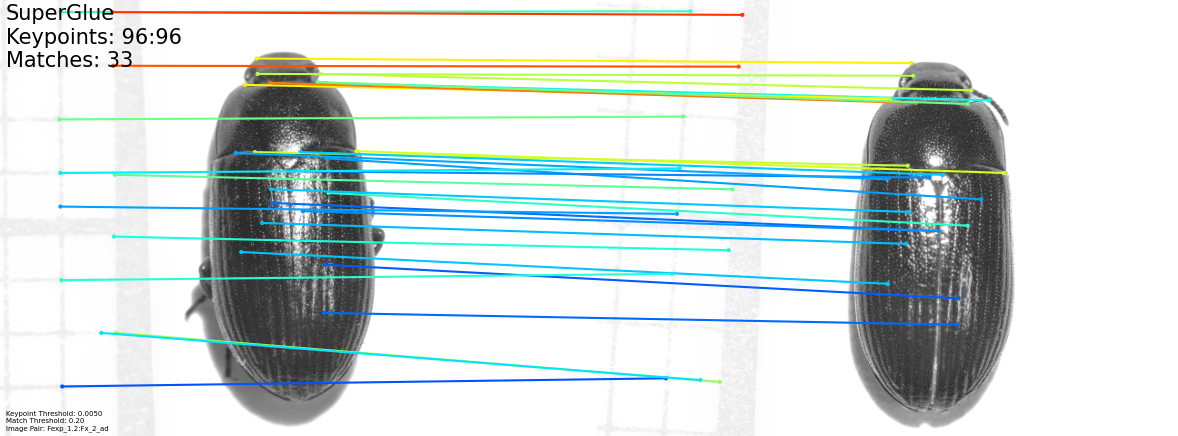
\includegraphics[width=1.0\linewidth]{pic/Fexp_1.2_Fx_2_ad_matches.png}
            \caption{Morphology of insects.}
        \end{figure}
    \end{frame}

    \begin{frame}{Application in urban intelligence}
        Spatio-Temporal Graph Convolutional Networks: A Deep Learning Framework for Traffic Forecasting \cite{yu2017spatio}.
        
        \begin{figure}[ht!]
            \centering
            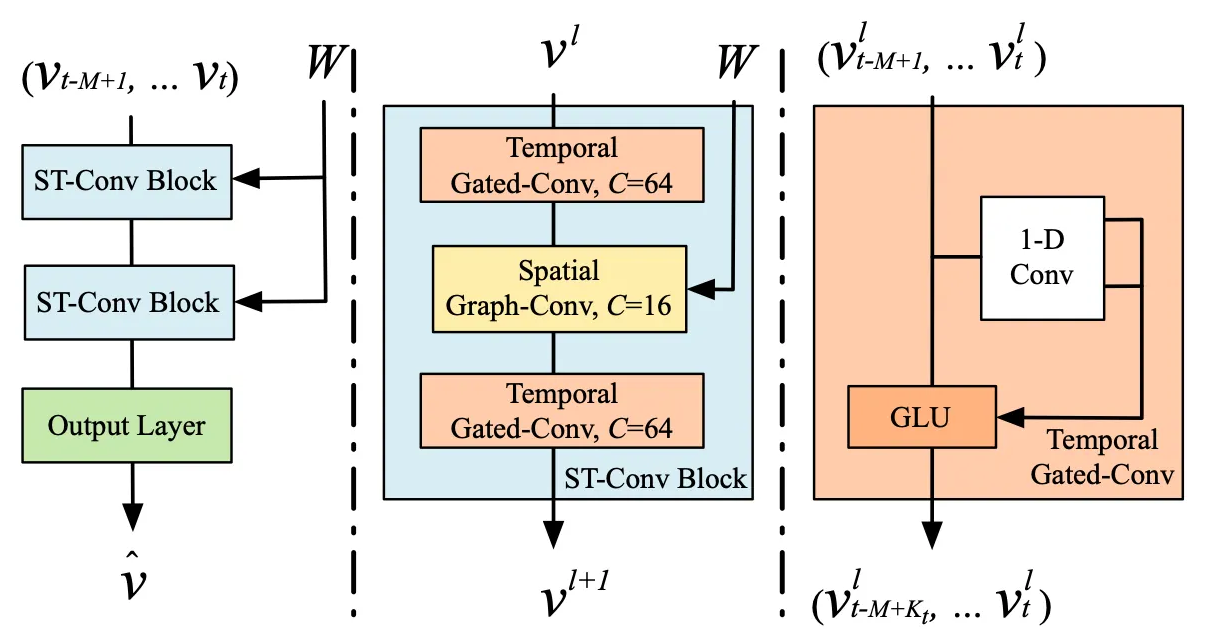
\includegraphics[width=0.8\linewidth]{pic/stgcn_model.png}
            \caption{STGCN scheme.}
        \end{figure}
    \end{frame}
    
    \begin{frame}{STGCN}
        \begin{figure}
            \centering
            % \includegraphics{}
            \animategraphics[width=0.85\textwidth, loop, autoplay]
            {15} % frame rate
            {pic/traffic/c389b48c98f34cce898d9c1baa2ed346LTsk9cwQTrdumRQT-} % path to figures
            {0} % start index
            {232} % end index
            \caption{Visualization of traffic. From \url{https://medium.com/stanford-cs224w/predicting-evolution-of-dynamic-graphs-7688eca1daf8}.}
            \label{fig:stgcn_example}
        \end{figure}
    \end{frame}

    \begin{frame}{Application in physic}
        Learning to Simulate Complex Physics with Graph Networks \cite{sanchez2020learning}.
        
        \begin{figure}[ht!]
            \centering
            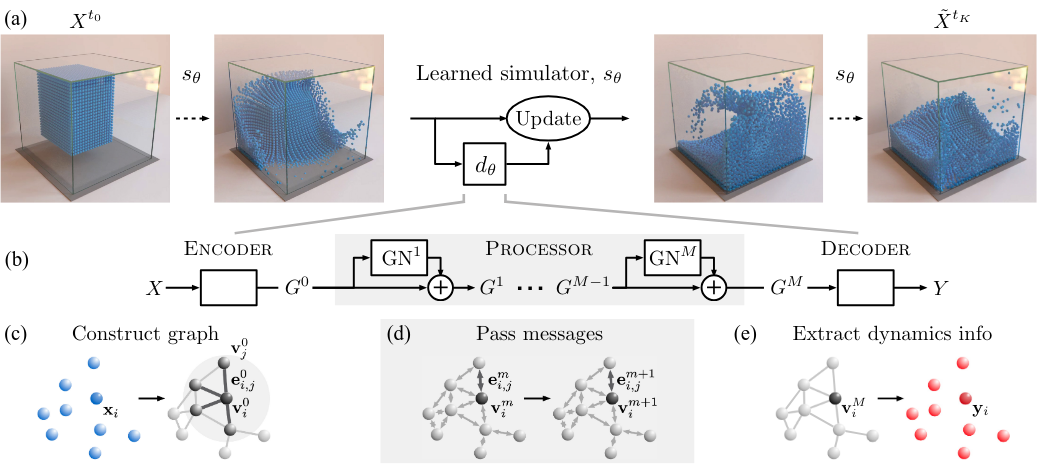
\includegraphics[width=0.9\linewidth]{pic/gns.png}
            \caption{GNS scheme.}
        \end{figure}
    \end{frame}
    
    \begin{frame}{GNS}
        \begin{figure}
            \centering
            % \includegraphics{}
            \animategraphics[width=0.85\textwidth, loop, autoplay]
            {10} % frame rate
            {pic/physics/96e5eb9cda094a5dacfe00a168965330KkJlbebmdYjuPPbO-} % path to figures
            {0} % start index
            {149} % end index
            \caption{Simulating complex physics. From \url{https://medium.com/stanford-cs224w/simulating-complex-physics-with-graph-networks-step-by-step-177354cb9b05}.}
            \label{fig:gns_example}
        \end{figure}
    \end{frame}

    \begin{comment}
    \begin{frame}{Practical example: GCN to node classification}
        \begin{figure}[ht!]
            \centering
            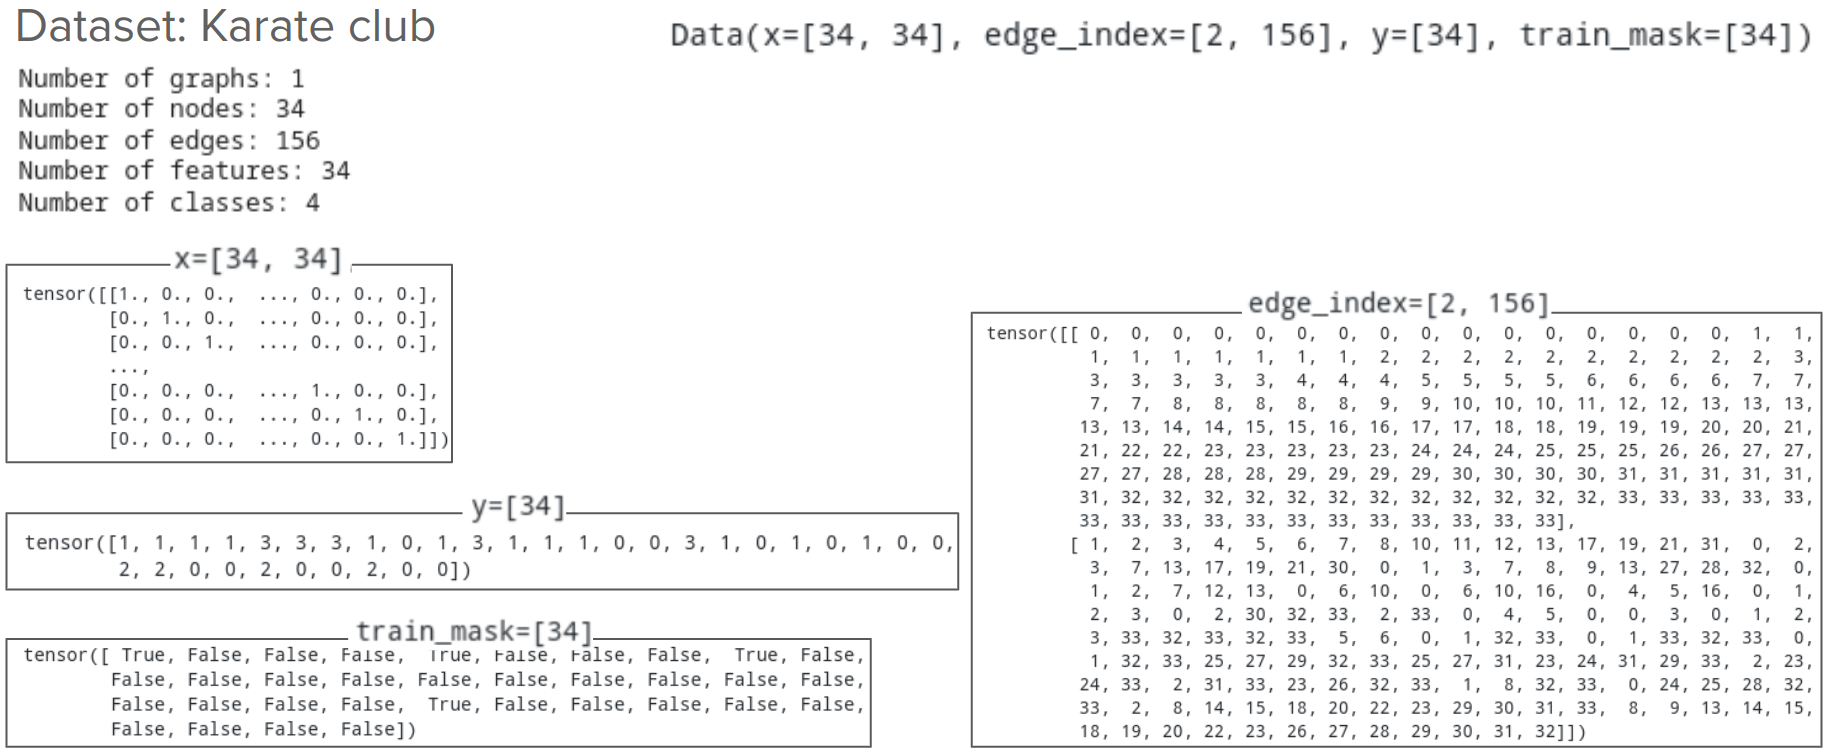
\includegraphics[width=1.0\linewidth]{pic/gcn_example.png}
            \caption{\scriptsize Karate club dataset.}
        \end{figure}
    \end{frame}
    \end{comment}

    \begin{comment}
    \begin{frame}{Practical example: GCN to node classification} 
        \url{https://drive.google.com/file/d/19ByHxX1AsqLiV3uqIoW5KLiuEDgCWdA5/view?usp=sharing}
    \end{frame}
    \end{comment}

    \begin{frame}{Application in bioinformatics} 
        \begin{figure}[ht!]
            \centering
            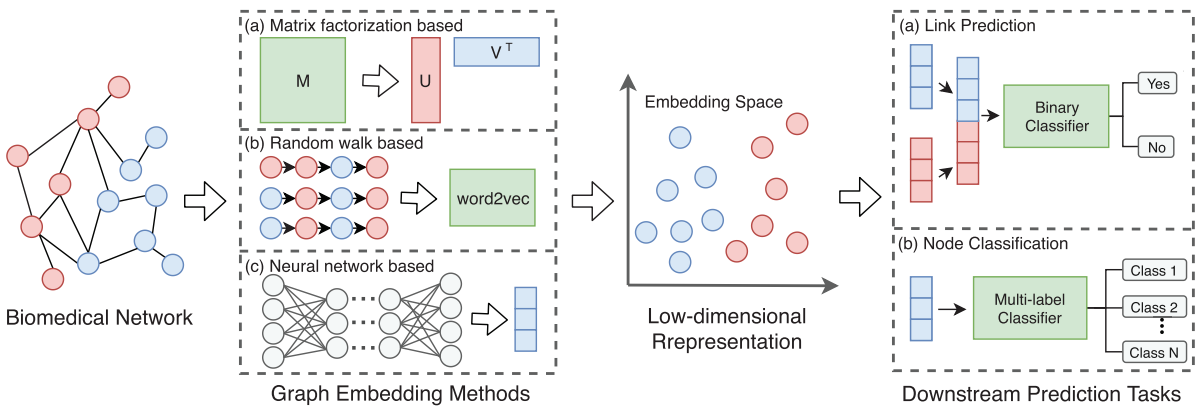
\includegraphics[width=1.0\linewidth]{pic/apply_graph_embedding.png}
            \caption{GNNs methods to biomedical tasks. Adapted from \cite{yue2020graph}.}
        \end{figure}
    \end{frame}
    
    \begin{frame}{Application in recommender systems}
        Uber Eats
        \begin{figure}[ht!]
            \centering
            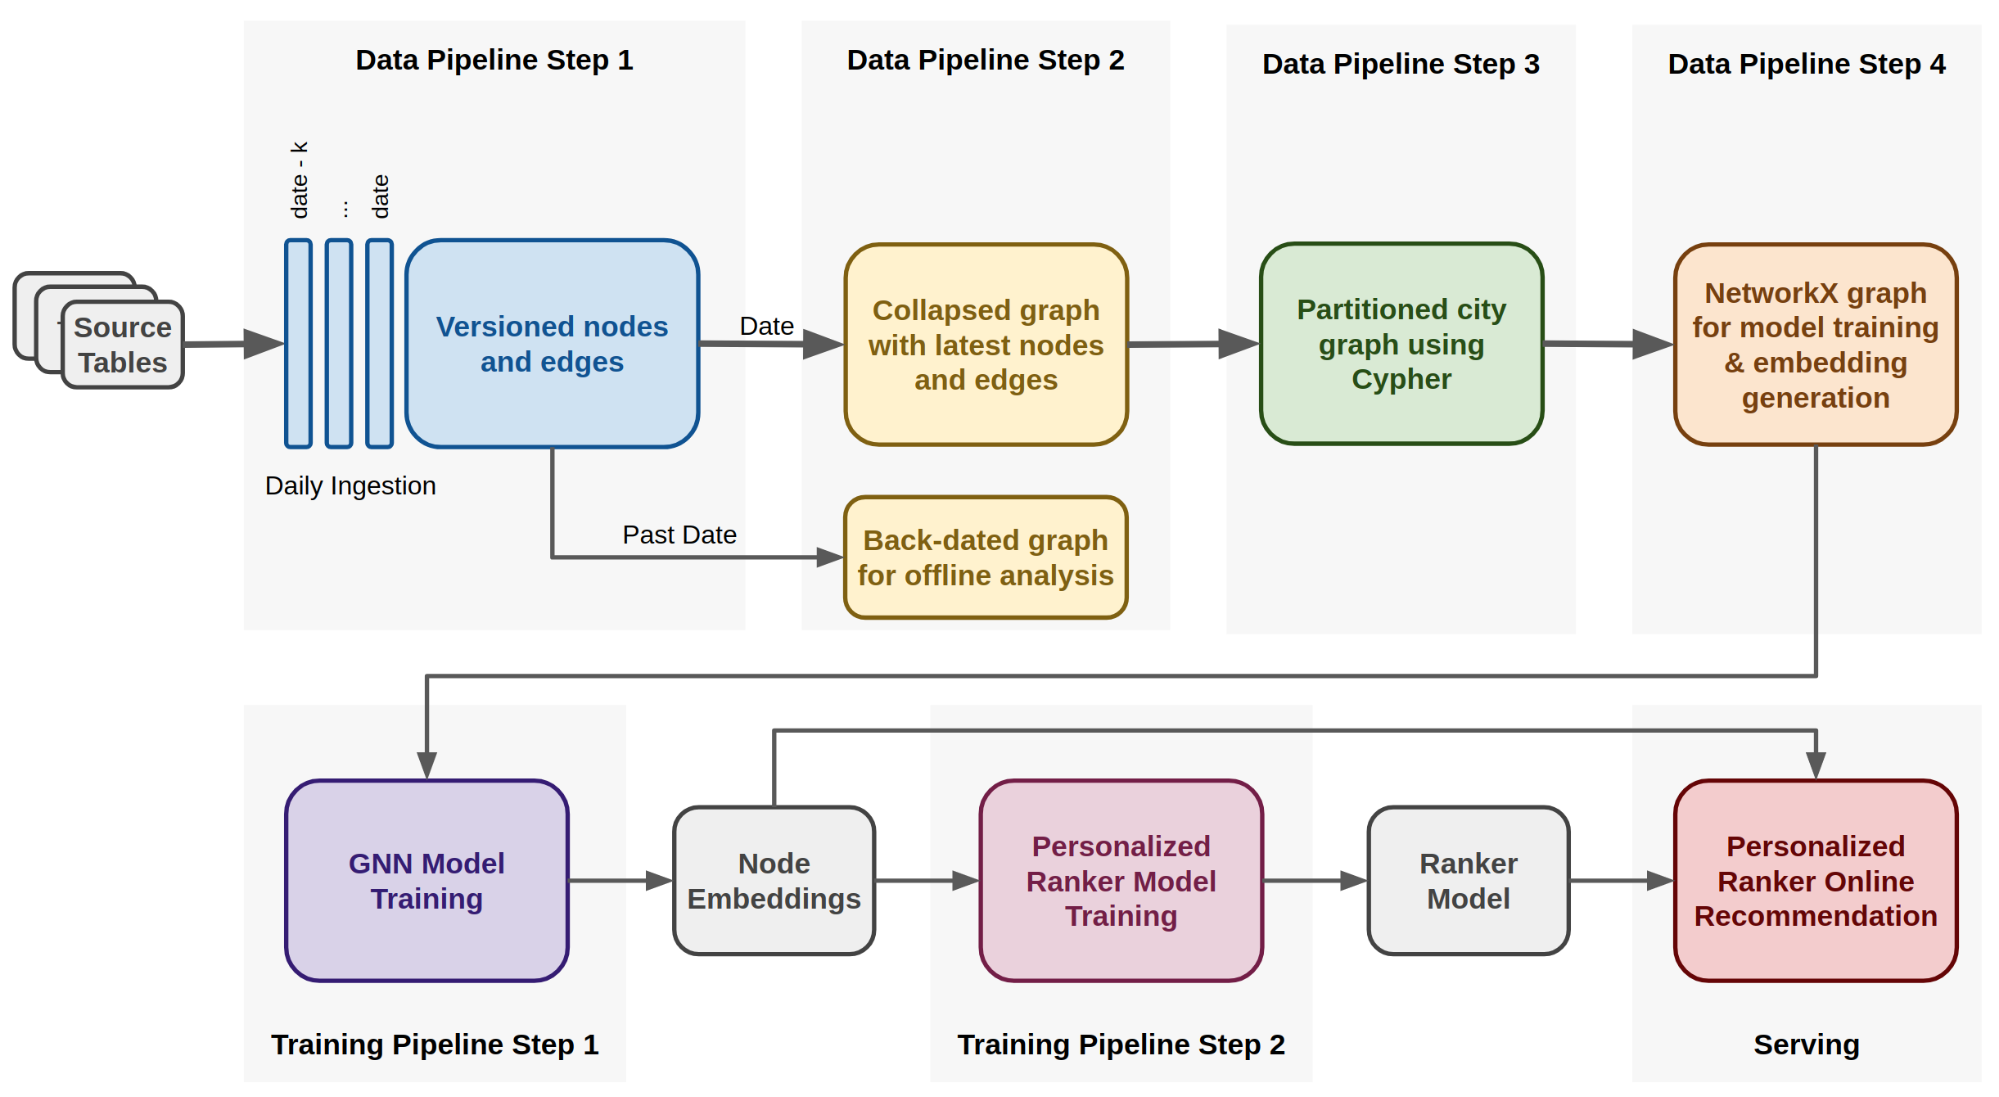
\includegraphics[width=0.9\linewidth]{pic/uber_model.png}
            \caption{Pipeline Uber eats. From \url{https://www.uber.com/en-CO/blog/uber-eats-graph-learning/}.}
        \end{figure}
    \end{frame}

    \begin{frame}{Uber Eats}
        \begin{figure}
            \centering
            % \includegraphics{}
            \animategraphics[width=0.35\textwidth, loop, autoplay]
            {5} % frame rate
            {pic/uber_eats/a733611516524151ebb9d28ad2c2ab68IaQ4dI3VB8Bs9CFt-} % path to figures
            {0} % start index
            {30} % end index
            \caption{Recommender systems app.}
            \label{fig:app_ubereats}
        \end{figure}
    \end{frame}

% \end{comment}

\section{Resources}
    \begin{frame}{Package, library, and framework}        
        \begin{figure}[ht!]
            \centering
            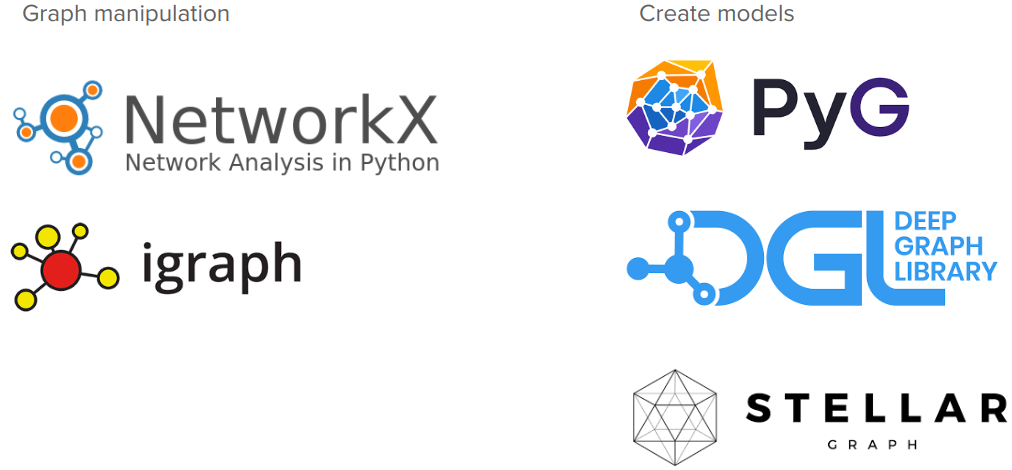
\includegraphics[width=0.9\linewidth]{pic/sources.png}
            \caption{\scriptsize Package, library, and framework.}
        \end{figure}               
    \end{frame}

    \begin{frame}{Books}        
        \begin{figure}[ht!]
            \centering
            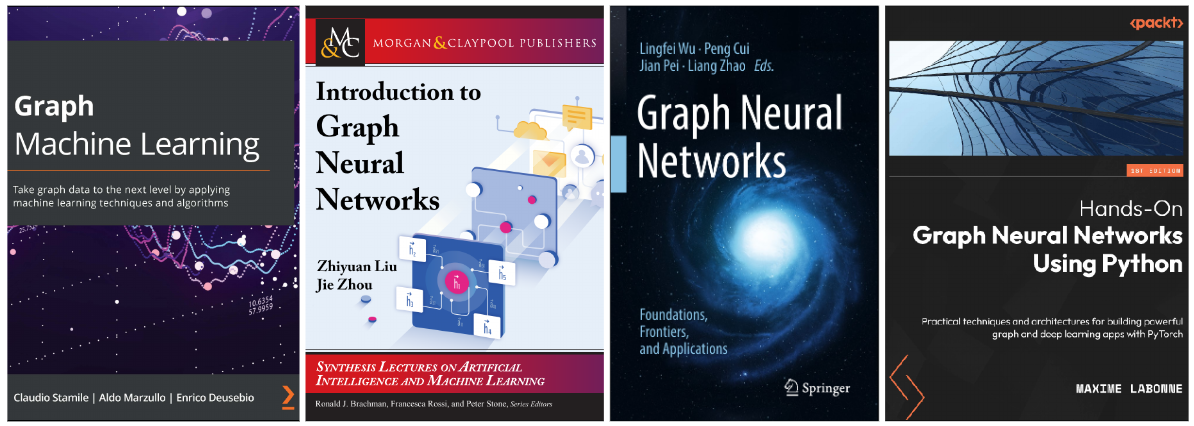
\includegraphics[width=1.0\linewidth]{pic/books_source.png}
            \caption{\scriptsize GNNs books.}
        \end{figure}               
    \end{frame}

    \begin{frame}{More learning}
        \begin{itemize}
            \item Courses
            \begin{itemize}
                \item CS224W: Machine Learning with Graphs \\ (\url{http://web.stanford.edu/class/cs224w/})
            \end{itemize}
            \item Tutorials
            \begin{itemize}
                \item PyTorch Geometric: Introduction by Example \\ (\url{https://pytorch-geometric.readthedocs.io/en/latest/notes/introduction.html})
            \end{itemize}
            \item Conferences
            \begin{itemize}
                \item Learning on Graphs \\ (\url{https://logconference.org/})
            \end{itemize}
        \end{itemize}
    \end{frame}

\begin{frame}[allowframebreaks]
    \bibliography{ref}
    % \bibliographystyle{unsrt}
    % \bibliographystyle{alpha}
    % If too many references, use this command to resize：
    \tiny\bibliographystyle{unsrt}
\end{frame}

\begin{frame}
    \begin{center}
        {\Huge\textit{Thank you for your attention!}}\\
        $\infty$ \\
        edwin.alvarez@unsaac.edu.pe\\
        \url{https://github.com/win7}
    \end{center}
    \begin{figure}[ht!]
        \centering
        
\includegraphics[width=0.2\linewidth]{pic/Laad_logo.png}
    \end{figure}
\end{frame}

%========================
% bibliography
%========================
% \input{ref.bib}

\end{document}